\documentclass{article}
\usepackage[T1]{fontenc}
\usepackage[utf8]{inputenc}
\usepackage[british]{babel}
\usepackage{amsthm}
\usepackage{amsfonts}
\usepackage{pgfplots}
\usepackage{amssymb}
\usepackage{amsmath}
\usepackage{mathtools}
\usepackage{color}
\usepackage{graphicx}
\usepackage{luatex85}
\usepackage[all]{xy}
\usepackage{geometry}
\usepackage{hyperref}
\usepackage{float}
\usepackage{tikz}
\usepackage{pst-plot}
\usepackage{ytableau}
\usepackage{microtype}
\usepackage{listings}
\usepackage[math]{iwona}
\usepackage{cmbright}

\renewcommand{\familydefault}{\sfdefault}

\geometry{a4paper,left=2cm,right=2cm,top=2cm,bottom=2cm}

\definecolor{codegreen}{rgb}{0,0.6,0}
\definecolor{codegray}{rgb}{0.5,0.5,0.5}
\definecolor{codepurple}{rgb}{0.58,0,0.82}
\definecolor{backcolour}{rgb}{0.95,0.95,0.92}

\lstdefinestyle{mystyle}{
	backgroundcolor=\color{backcolour},
	commentstyle=\color{codegreen},
	keywordstyle=\color{magenta},
	numberstyle=\tiny\color{codegray},
	stringstyle=\color{codepurple},
	basicstyle=\ttfamily\footnotesize,
	breakatwhitespace=false,
	breaklines=true,
	captionpos=b,
	keepspaces=true,
	numbers=left,
	numbersep=5pt,
	showspaces=false,
	showstringspaces=false,
	showtabs=false,            
	tabsize=2
}

\lstset{style=mystyle}

\usetikzlibrary{decorations.pathreplacing}

\pgfplotsset{compat=1.18}

\newcommand{\tikznode}[3][inner sep=0pt]{\tikz[remember
picture,baseline=(#2.base)]{\node(#2)[#1]{$#3$};}}

\ytableausetup{smalltableaux}

\makeatletter
\renewcommand*\env@matrix[1][*\c@MaxMatrixCols c]{%
  \hskip -\arraycolsep
  \let\@ifnextchar\new@ifnextchar
  \array{#1}}
\makeatother
\makeatletter
\DeclareRobustCommand{\pns}{\mathrel{\text{$\m@th\proper@ideal$}}}
\newcommand{\proper@ideal}{%
  \ooalign{$\lneq$\cr\raise.22ex\hbox{$\lhd$}\cr}%
}
\makeatother

\SelectTips{eu}{}
\setlength{\fboxsep}{0pt}
\setlength\parskip{0.3em}
\setlength{\parindent}{0 pt}

\newcommand{\F}{\mathbb{F}}
\newcommand{\N}{\mathbb{N}}
\newcommand{\Z}{\mathbb{Z}}
\newcommand{\Q}{\mathbb{Q}}
\newcommand{\R}{\mathbb{R}}
\newcommand{\C}{\mathbb{C}}
\newcommand{\p}{\mathbb{P}}
\newcommand{\A}{\mathbb{A}}
\newcommand{\Mod}{\text{ mod }}
\newcommand{\Char}{\operatorname{char}}
\newcommand{\im}{\operatorname{im}}
\newcommand{\vol}{\operatorname{vol}}
\newcommand{\Gal}{\operatorname{Gal}}
\newcommand{\Res}{\operatorname{Res}}
\newcommand{\Hom}{\operatorname{Hom}}
\newcommand{\End}{\operatorname{End}}
\newcommand{\la}{\left\langle}
\newcommand{\ra}{\right\rangle}

\theoremstyle{definition}

\newtheorem{defn}{Definition}[subsection]
\newtheorem{prop}[defn]{Proposition}
\newtheorem{thm}[defn]{Theorem}
\newtheorem{lemma}[defn]{Lemma}
\newtheorem{coro}[defn]{Corollary}
\newtheorem{example}[defn]{Example}
\newtheorem{exe}[defn]{Exercise}
\newtheorem{claim}[defn]{Claim}
\newtheorem{conj}[defn]{Conjecture}
\newtheorem*{remark}{Remark}
\newtheorem*{notation}{Notation}

\title{MATH70064 Elliptic curves :: Lecture notes}
\author{Lecturer: Yanki Lekili}
\date{Last edited: \today}

\begin{document}

\maketitle
\thispagestyle{empty}

\tableofcontents
\thispagestyle{empty}
\newpage
\setcounter{page}{1}

\begin{flushright}
\textit{Week 1, lecture 1, 3rd October}
\end{flushright}

\subsection*{References}
\begin{itemize}
\item Cassels. Lectures on elliptic curves
\item Silverman-Tate. Rational points on elliptic curves
\end{itemize}

\section{Introduction}
\subsection{Notation and basic definitions}
$k$, field, e.g. $\Q, \R, \C, \F_p, \Q_p, \Q(i), \Q(\sqrt 3)$.

$k[x,y]$ or $k[x,y,z]$, polynomials. Degree 2 ones are \textit{conics} (usually denoted $Q$), degree 3 are \textit{cubics}.

An \textit{elliptic curve} $E: y^2+a_1xy+a_3y=x^3+a_2x^2+a_4x+a_6$ where $a_1,a_2,a_3,a_4,a_6\in k$. If $\Char k\neq 2$ or 3 then it can be written as $y^2=x^3+ax+b$ by change of variables where $a,b\in k$ and $\Delta=4a^3+27b^2\neq 0$.

$E(\Q):=\{(x,y)\in \Q\times \Q:y^2=x^3+ax+b\}=\Z^r\times E(\Q)_{\text{torsion}}$ is a finitely generated abelian group where $r$ is called the \textit{rank} of the elliptic curve.

\subsection{Big idea 1: Geometric method of constructing solutions}

\begin{example}
\label{example:acircletobeginwith}
One can think of the solutions of $x^2+y^2=1$ over $\R$ as a circle. What about over $\Q$? The solutions can be written down as
\[
x=\frac{1-t^2}{1+t^2},\quad y=\frac{2t}{1+t^2}\quad \text{where } t\in\Q\cup\{\infty\}
\]
by parametrise by connecting $(-1,0)$ and $(0,t)$.

\begin{center}
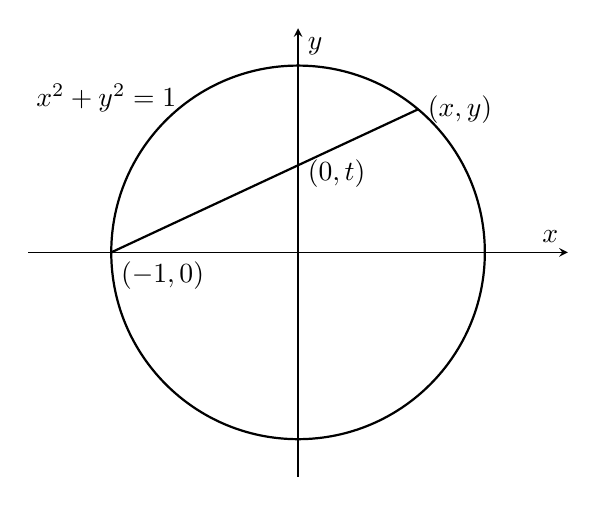
\begin{tikzpicture}
\begin{axis}[axis equal,axis lines=middle,xmin=-1.2,xmax=1.2,ymin=-1.2,ymax=1.2,xtick=\empty,ytick=\empty,xlabel=$x$,ylabel=$y$]
\draw[thick] (-1,0) -- (0.6427876,0.766);
\draw[thick] (0,0) circle[radius=1];
\draw (-0.6,0.7) node[anchor=south east] {$x^2+y^2=1$};
\draw (-1,0) node[anchor=north west] {$(-1,0)$};
\draw (0.6427876,0.766) node[anchor=west] {$(x,y)$};
\draw (0,0.42261826174) node[anchor=west] {$(0,t)$};
\end{axis}
\end{tikzpicture}
\end{center}
\end{example}

\begin{example}
\label{example:CTP1stencounter}
$E:y^2+y=x^3-x$. There's an inductive way to find a list of its solutions which may be infinite (and we shall know for sure later): we first notice $(0,0)$ as a trivial solution, at which the tangent line is of the equation $y=-x$, which intersects the curve at $(2,-3)$.

\begin{center}
\begin{tikzpicture}
\begin{axis}[axis lines=middle,xmin=-1.2,xmax=3,ymin=-4,ymax=2,xtick=\empty,ytick=\empty,xlabel=$x$,ylabel=$y$,legend pos=south west]
	
\addplot[smooth,samples=100,no markers,thick,blue!25] {-x};
\addplot[smooth,samples=100,no markers,thick,blue!50] {-2*x+1};
\addplot[smooth,samples=100,no markers,thick,blue!75] {-11*x/5+7/5};

\addplot[thick,smooth] table {data.dat};

\node[circle,fill,inner sep=1.5pt,label={260:{$(0,0)$}}] at (0,0) {};
\node[circle,fill,inner sep=1.5pt,label={0:{$(1,-1)$}}] at (1,-1) {};
\node[circle,fill,inner sep=1.5pt,label={180:{$(2,-3)$}}] at (2,-3) {};
\node[circle,fill,inner sep=1.5pt,label={0:{$\left(\frac{21}{25},-\frac{56}{125}\right)$}}] at (21/25,-56/125) {};

\legend{$y=-x$,$y=-2x+1$,$y=-\frac{11x}{5}+\frac75$}
\end{axis}
\end{tikzpicture}
\end{center}

One proceeds successively (recall Newton method) to derive more solutions as shown above. The calculation can be done efficiently by the computer algebra system \texttt{PARI/GP}:

\begin{lstlisting}
? E = ellinit([0,0,1,-1,0])
%1 = [0, 0, 1, -1, 0, 0, -2, 1, -1, 48, -216, 37, 110592/37, Vecsmall([1]), [Vecsmall([128, 1])], [0, 0, 0, 0, 0, 0, 0, 0]]
? P = [0,0]
%2 = [0, 0]
? Q = ellmul(E,P,-2)
%3 = [1, -1]
? R = ellmul(E,Q,-2)
%4 = [2, -3]
? S = ellmul(E,R,-2)
%5 = [21/25, -56/125]
\end{lstlisting}
\end{example}

\subsection{Big idea 2: Local to global}
Given an equation over $\Q$, we can suppose it has an $\Z$-form by multiplying the common denominator, and then reduce modulo $p$ for prime $p$ or $q=p^k$. Sometimes by writing $p=\infty$ we consider the equation over $\R$. Fields like $\Q_p$ and $\R$ are called \textit{local}. Behind this is \textit{Hasse principle}, ``the idea that one can find an integer solution to an equation by using the Chinese remainder theorem to piece together solutions modulo powers of each different prime number''.

\begin{example}
We claim $x^2+y^2=2(x+y)z+z^2$ does not have a solution in $\Q_2$.

Indeed, rewrite the equation by $t=x+y+z$ as $2x^2+2xy+2y^2=t^2$. Since it's homogeneous, it suffices to show there's no integer solutions and one can assume $\gcd(x,y,t)=1$. $t^2$ is divisible by 2 so divisible by 4, hence $x^2+xy+y^2=0\Mod 2\iff x=y=0\Mod 2$, but then $2\mid\gcd(x,y,t)$, a contradiction.
\end{example}

But the Hasse principle doesn't always hold, e.g. an example of Selmer, $3x^3+4y^3+5z^3=0$ has solutions over all $\Q_p$ including $p=\infty$ but no nontrivial $\Q$ solution.

\subsection{Big idea 3: Descent}
\begin{example}
\begin{thm}[Fermat]
	For a right triangle with sides of rational number, its area is not a square, i.e. if $a,b,c\in\Q$ and $c^2=a^2+b^2$ then $\nexists a\in\Q:a^2=\frac{ab}{2}$.
\end{thm}
\begin{proof}[Proof by descent]
Without loss of generality, assume $a,b,c\in\Z$ are pairwise coprime. For contradiction, suppose $\frac{ab}{2}$ is a square. Recall that Pythagorean triples are parametrised by $a=p^2-q^2,b=2pq,c=p^2+q^2$ where $\gcd(p,q)=1$ and $p-q$ is odd. Hence
\[
\frac{ab}{2}=pq(p+q)(p-q)
\]
so
\[
\exists x,y,u,v:p=x^2,q=y^2,p+q=u^2,p-q=v^2
\]
where $u,v$ are odd and coprime. Note that
\[
\left(\frac{u-v}{2}\right)^2+\left(\frac{u+v}{2}\right)^2=x^2
\]
where $\frac{u-v}{2},\frac{u+v}{2}\in\Z$ by above, hence $x\in\Z$. Now
\[
\frac{\left(\frac{u-v}{2}\right)\left(\frac{u+v}{2}\right)}{2}<\frac{ab}{2}
\]
where the left hand side is a square of an integer. We have a right triangle with a strictly smaller area that's also a square, but the process cannot continue infinitely, a contradiction.
\end{proof}
\end{example}

\section{$p$-adic numbers}
\begin{defn}
A $p$\textit{-adic integer} $x\in\Z_p$ is a formal solution to system of congruences $x\equiv x_n\Mod p^n$ ($n=1,2,\ldots$) such that $x_n\equiv x_{n+1}\Mod p^n$.
\end{defn}
\begin{defn}
A \textit{norm} on a field \textit{k} is a function $|\cdot|:k\rightarrow \R_{\geq 0}$ such that $|x|=0\iff x=0$, $|xy|=|x||y|$ and $|x+y|\leq|x|+|y|$.
\end{defn}
One can define a topology from the metric induced by a norm ($d(x,y)=|x-y|$).

In this module we focus on the field $\Q$.
\begin{defn}
The $p$\textit{-adic norm} $|\cdot|_p$ on $\Q$ is defined by the following: given $r\in\Q$, write it as $p^\rho \frac{a}{b}$ where $a,b,\rho\in\Z$ and $p\nmid a,b$, then $|r|_p=p^{-\rho}$.
\end{defn}

$p$-adically speaking, a number is \textit{small} when it's divisible by a high power of $p$.

\begin{prop}
$p$-adic norm is a norm.
\end{prop}
\begin{proof}
The first two conditions are obviously satisfied, so it remains to see $|r+s|_p\leq |r|_p+|s|_p$. Write
\[
r=p^\rho \frac{a}{b},\quad s=p^\sigma\frac{c}{d},\quad r+s=p^\rho\frac{ad+p^{\sigma-\rho}cb}{bd}
\]
assuming $\sigma\geq\rho$, hence $|r+s|_p\leq p^{-\rho}\leq \max\{|r|_p,|s|_p\}$ (this is the ultrametric inequality).
\end{proof}

\begin{flushright}
\textit{Week 2, lecture 1, 8th October}
\end{flushright}

\begin{lemma}
\label{lemma:isosceles}
Let $|\cdot|:k\rightarrow \R_{\geq 0}$ be a norm that satisfies the ultrametric inequality. If $|x|<|y|$ then $|x-y|=|y|$ (every triangle is isosceles).
\end{lemma}
\begin{proof}
One has $|x-y|\leq \max\{|x|,|y|\}=|y|$ and $|y|=|y-x+x|\leq \max\{|y-x|,|x|\}=|y-x|$.
\end{proof}

\begin{exe}
Show that if we change the definition of $p$-adic norm by replacing the $p$ be a composite number $n$, then it's not a norm.
\end{exe}

Recall the definition of a Cauchy sequence: $(x_n)_{n\geq 1}$ is Cauchy if $\forall\varepsilon>0,\ \exists k:|x_n-x_m|<\varepsilon\ \forall n,m>k$. Note that 5-adically, the sequence $x_1=3,x_2=34,x_3=334,x_4=3334,\ldots$ is Cauchy since the differences become increasingly highly divisible by 5, and the limit is $\frac23$ since $\left|x_n-\frac23\right|_5\rightarrow 0$ (since $|3x_n-2|_5\rightarrow 0$).

In the same spirit that Cauchy sequences complete $\Q$ to $\R$, $\Q$ is also $p$-adically incomplete. Construct a sequence $(x_n)$ of integers by $x_n^2+1\equiv 0\Mod 5^n$ and $x_{n+1}\equiv x_n\Mod 5^n$. Choose $x_1=2$ and suppose $x_n$ is constructed. By induction it suffices to show $x_{n+1}$ can be constructed to see this sequence is well-defined. Write $x_n^2+1=5^nc$ and $x_{n+1}=x_n+b5^n$ such that $(x_n+b5^n)^2+1\equiv 0\Mod 5^{n+1}$. Hence one needs to solve $2x_nb+c\equiv 0\Mod 5$, which is indeed solvable since $5\nmid x_n$.

Now the limit $x$ must satisfy $x^n+1=0$, which doesn't have a rational solution. In this sense we give another definition of $p$-adic numbers:
\begin{defn}
$\Q_p$ is the completion of $\Q$ with respect to $|\cdot|_p$.
\end{defn}

\begin{notation}
$\mathcal C:=\{(x_n)_{n\geq 1}:x_n\in k,(x_n)\text{ Cauchy}\}$.

$\mathcal I:=\{(x_n)_{n\geq 1}\in\mathcal C:\lim_{n\rightarrow\infty} x_n=0\}$.

$\widehat k:=\mathcal C/\mathcal I$, the equivalence classes of Cauchy sequences with the same limit.

It's clear that $\mathcal C$ is a commutative ring (with $(x_n)\pm (y_n)=(x_n\pm y_n)$ and $(x_n)(y_n)=(x_ny_n)$ as expected) and $\mathcal I$ is an ideal. We claim $\mathcal I$ is maximal and we shall see why after the following lemma.
\end{notation}

\begin{lemma}
Let $(x_n)\in \mathcal C\backslash \mathcal I$, then $\exists n_0\geq 1: |x_n|=|x_{n_0}| \ \forall n\geq n_0$.
\end{lemma}

\begin{proof}
Since $\lim_{n\rightarrow\infty} x_n\neq 0,\ \exists \varepsilon>0$ such that for any $x_N$ one can find $x_{n(N)}$ such that $n(N)>N$ and $|x_{n(N)}|>\varepsilon$. Now by definition of a Cauchy sequence, $\exists M\geq 1:|x_n-x_m|<\varepsilon \ \forall n,m\geq M$. Then, for all $n\geq n(M)>m$ one has $|x_{n(M)}|>\varepsilon>|x_n-x_{n(M)}|$, and by \ref{lemma:isosceles} one has $|x_{n(M)}|=|x_n| \ \forall n\geq n(M)$.
\end{proof}

Hence for all $(x_n)\in\mathcal C\backslash\mathcal I$, one can define
\[
(y_n)=\left\{\begin{aligned}
0 &\quad n<n_0 \\
\frac{1}{x_n}&\quad n\geq n_0
\end{aligned} \right.
\]
where $n_0$ is the number we proved exists above and $x_n$ is the limit of $(x_n)$. Then $(x_n)(y_n)=1_{\mathcal C/\mathcal I}$ so $\mathcal I$ is maximal. One also the norm $|\cdot|:\widehat k\mapsto\R_{\geq 0}:(x_n)\rightarrow\lim_{n\rightarrow\infty}|x_n|$ on $\widehat k$.

\begin{lemma}
The field embedding $k\rightarrow\widehat k$ by $x\mapsto (x)_{n\geq 1}$ is dense, i.e. the closure of the image of $k$ in $\widehat k$ is $\widehat k$. (Recall that $\Q$ is dense in $\R$).
\end{lemma}
\begin{proof}
Let $(x_n)\in\widehat k$ and $\varepsilon>0$. We want to show that $\exists (y)$ in the image of the embedding such that $|(x_n)-(y)|<\varepsilon$, but this follows immediately from definition of Cauchy: choose $N$ such that $n,m\geq N\implies|x_n-x_m|<\varepsilon$ and take $(y)=(x_N)$.
\end{proof}

\begin{lemma}
$\widehat k$ is complete, i.e. every Cauchy sequence in $\widehat k$ has its limit in $\widehat k$.
\end{lemma}
\begin{proof}
Let $(x_n)$ be a Cauchy sequence (of equivalence classes of Cauchy sequences) in $\widehat k$. By lemma above, $\forall n\geq 1 \exists y_n\in k:|x_n-y_n|<\frac1n$. We claim $y=(y_n)\in\widehat k$ is Cauchy, which is clear from equation (1), and $\lim_{n\rightarrow\infty}x_n=y$, clear from (2).

\[
|y_m-y_n|\leq |y_m-x_m|+|x_m-x_n|+|x_n-y_n|=\frac1m+\frac1n+|x_m-x_n| \tag{1}
\]
\[
|x_n-y|\leq |x_n-y_n|+|y_n-y|<\frac1n+|y_n-y|. \tag{2}
\]
\end{proof}

\begin{flushright}
\textit{Week 2, lecture 2, 10th October}
\end{flushright}

\begin{remark}
In this module we focus on the field $\Q$ with the $p$-adic norm $|\cdot|_p$ which by above completes to $\widehat\Q=\Q_p$. In this sense, $p$-adic integers are
\[
\Z_p:=\{x\in\Q_p:|x|_p\leq 1\}.
\]
Note that $|\alpha|_p,|\beta|_p\leq 1\implies |\alpha\beta|_p\leq 1$ and $|\alpha+\beta|_p\leq 1$, which verifies $\Z_p$ is indeed a ring. One has the inclusion matrix
\[
\xymatrix@C=0.3pc @R=0.3pc{
	\Z_p & \subset & \Q_p \\
	\rotatebox{90}{\subset} & & \rotatebox{90}{\subset} \\
	\Z & \subset & \Q
}
\]
where
\[
\Z_p\cap\Q=\Z_{(p)}:=\left\{\frac{u}{v}\in\Q:p\nmid v\right\},\quad\text{localisation of }\Z\text{ at prime ideal }(p)
\]
and $\Z_p^\ast=\{x\in\Z_p:|x|_p=1\}$.

Note that if $x\in\Q_p$ then either $x\in\Z_p$ or $x^{-1}\in\Z_p$ since either $p^{-\rho}\geq 1\implies p^{\rho} \leq 1$.

$\Z_p$ has an ideal $(p)=\{x\in\Z_p:|x|_p<1\}$. It's maximal since $\Z_p/(p)=\F_p$, a field, and it's the unique maximal ideal since $\Z_p\backslash(p)=\Z_p^\ast$. Hence $\Z_p$ is local.

Note that $\frac1p\notin\Z_p$ since $\left|\frac1p\right|_p=p>1$, and in fact $\Q_p=\Z_p\left[\frac1p\right]$, i.e. $\Q_p$ is the field of fractions of $\Z_p$.
\end{remark}

\subsection{Series expansion on $\Q_p$}
\begin{defn}
We define a \textit{series} $\sum_{n=0}^\infty\beta_n\in\Q_p$ in the usual way as $\lim_{N\rightarrow\infty}\sum_{n=0}^N\beta_n$.
\end{defn}
\begin{lemma}
$\sum_{n=0}^\infty\beta_n$ converges $\iff\beta_n\rightarrow 0$.
\end{lemma}
A well-known counterexample in the usual norm is the harmonic series.
\begin{proof}
$\implies$ is obvious by what we've seen in real analysis. Now suppose $\beta_n\rightarrow 0$ and $M<N$, then by induction on the ultrametric inequality
\[
\left|\sum_{n=0}^N\beta_n-\sum_{n=0}^M\beta_n\right|_p=\left|\sum_{n=M+1}^N\beta_n\right|_p\leq \max_{M<N\leq N} |\beta_n|_p,
\]
so $\impliedby$ is clear as well.
\end{proof}

\begin{lemma}
\label{lemma:padicasseries}
$p$-adic integers are precisely $\alpha=\sum_{n=0}^\infty a_np^n$ where $a_n\in\{0,1,\ldots,p-1\}$.
\end{lemma}
\begin{proof}
First observe that by lemma above $\alpha$ indeed converges since $|p^n|_p=p^{-n}\rightarrow 0$.

We know $\Q$ is dense in $\Q_p$, in particular $\exists b\in\Q:|\alpha-b|_p<1$. Now $|\alpha|_p\leq 1$ by definition, so $|b|_p\leq 1$. We can then write $b=\frac{r}{s}$ where $(r,s)=1$, so that $p\nmid s$. Hence we can find a unique $a_0\in\{0,\ldots,p-1\}:sa_0-r\equiv 0\Mod p$, i.e. $b-a_0$ is divisible by $p$, hence $|b-a_0|_p<1$, so $|\alpha-a_0|_p<1$, so again one can find $\alpha_1:\alpha=a_0+p\alpha_1$ where $\alpha_1\in\Z_p$ since $|p\alpha_1|_p=|\alpha-a_0|_p<1$. One proceeds inductively (keeps separating the part that's not divisible by $p,p^2,\ldots$) with $\alpha_1$ as the new $\alpha$.
\end{proof}

\begin{coro}
$p$-adic numbers are precisely $\alpha=\sum_{n\geq -T}a_np^n$ where $a_{-T}\neq 0,a_n\in\{0,1,\ldots,p-1\}$.
\end{coro}
\begin{proof}
If $\alpha\in\Q_p$ then write $|\alpha|_p=p^T$, so $|p^T\alpha|_p=1$, i.e. $p^T\alpha\in\Z_p$ and then one uses the lemma above.
\end{proof}

\begin{coro}
$\Z$ is dense in $\Z_p$.
\end{coro}

\begin{example}
\texttt{GP} can do $p$-adic arithmetic:

\begin{lstlisting}
? x = 3^-1 + 2 + 2*3 + 3^2 + 3^3 + 3^4 + O(3^5)
%1 = 3^-1 + 2 + 2*3 + 3^2 + 3^3 + 3^4 + O(3^5)
? y = 1/4 + O(3^5)
%2 = 1 + 2*3 + 2*3^3 + O(3^5)
? x*y
%3 = 3^-1 + 1 + 3 + 3^3 + O(3^4)
? x+y
%4 = 3^-1 + 2*3 + 2*3^2 + 2*3^4 + O(3^5)
\end{lstlisting}
\end{example}

\begin{exe}
\begin{enumerate}
\item Show that $\alpha\in\Q_p$ has a finite expansion $\iff\alpha$ is a positive rational integer with denominator a power of $p$.
\item Show that $\alpha\in\Q_p$ is in $\Q\iff$ it's eventually periodic.
\end{enumerate}
\end{exe}

\begin{flushright}
\textit{Week 2, lecture 3, 11th October}
\end{flushright}

We are now interested in solutions to polynomial equations in $\Q_p$.

\begin{lemma}
Let $\epsilon\in\Z_p$ be a unit where $p\neq 2$. The equation $x^2=\epsilon$ has a solution $x\in\Q_p \iff \epsilon$ is a square mod $p$. (Note that if $x$ is a solution then $|x|_p$, so in fact $x\in\Z_p$.)
\end{lemma}
\begin{proof}
Suppose $x\in\F_p:x^2=\epsilon\Mod p$. We want to construct from this a $p$-adic solution.

We do this inductively: let $\alpha_1=x$ and construct $\alpha_n$ by $|\alpha_n^2-\epsilon|_p\leq p^{-n},\ |\alpha_{n+1}-\alpha_n|_p\leq p^{-n}$ (i.e. $\alpha_n^2$ is very close to $\epsilon$, $\alpha_{n+1}$ is very close to $\alpha_n$). The solution would then be $\lim_{n\rightarrow\infty}\alpha_n$ since it is Cauchy.

It remains to see why such $\alpha_{n+1}$ exists if one has constructed $\alpha_n$. We simply set $\alpha_{n+1}=\alpha_n+p^n\beta$ and find $\beta$, then
\[
\alpha_{n+1}^2\equiv \alpha_n^2+2\alpha_np^n\beta+p^{2n}\beta^2\equiv \alpha_n^2+2\alpha_np^n\beta\Mod p^{n+1}
\]
where $p^n\mid \alpha_n^2-\epsilon$. Hence one can rearrange the above as (this is where $p=2$ fails)
\[
2\alpha_n\beta\equiv \frac{\epsilon-\alpha_n^2}{p^n}\Mod p.
\]
\end{proof}

\begin{lemma}
\label{lemma:squaresinQ2}
Let $\epsilon\in\Z_2$ be a unit. The equation $x^2=\epsilon$ has a solution $x\in\Q_2 \iff \epsilon\equiv 1\Mod 8$.
\end{lemma}

\begin{exe}
Let $p$ be a prime such that $p\equiv 2\Mod 3$. Show that $x^3=a$ has a solution $x\in\Z_p$ if $p\nmid a$.

Show that there is no 7-adic number $x=2+y$ where $|y|_7\leq 7^{-1}:x^3+x^2-2x-1=0$.
\end{exe}

\begin{lemma}[Hensel's]
\label{lemma:Hensel}
Let $f=\sum_{i=0}^n a_i x^i\in\Z_p[x]$. Suppose $x_0\in\Z_p$ satisfies $|f(x_0)|_p<|f'(x_0)|_p^2$ where $f'(x)=\sum_{i=1}^n ia_i x^{i-1}$, the formal derivative. Then there exists a unique root $x$ of $f$ in $\Z_p$ satisfying $|x-x_0|_p<|f'(x_0)|_p$.

A stronger and more standard assumption: consider the reduction homomorphism $\overline{\phantom{\phi}}:\Z_p\rightarrow\Z_p/(p)$ to the residue finite field and write $\overline f=\sum_{i=0}^n \overline{a_i}x^i\Z_p/(p)[x]$. Suppose $\exists\overline{x_0}\in\F_p:\overline f(\overline{x_0})=0$ and $\overline{f}'(\overline{x_0})\neq 0$ (i.e. $x_0$ is a simple root of $\overline f$).
\end{lemma}

\begin{proof}
First observe that by assumption and since $f\in\Z_p[x],x_0\in\Z_p$,
\[
\frac{|f(x_0)|_p}{|f'(x_0)|_p}< |f'(x_0)|_p\leq 1,
\]
and we write $y_0=\frac{f(x_0)}{f'(x_0)}$ so that $|y_0|_p<1$ and $f(x_0)+y_0f'(x_0)=0$.

Define polynomials $f_1,f_2,\ldots\in\Z_p[x]$ by
\[
f(x+y)=f(x)+f_1(x)y+f_2(x)y^2+\cdots
\]
and consider $f(x_0+y_0)$. By the ultrametric inequality and assumption, one has
\[
|f(x_0+y_0)|_p\leq\max_{j\geq 2} \left|f_j(x_0)y_0^j\right|_p\leq |y_0|_p^2=\frac{|f(x_0)|_p^2}{|f'(x_0)|_p^2}<|f(x_0)|_p
\]
since $f_j(x_0)\in\Z_p\implies |f_k(x_0)|_p\leq 1$; i.e. $x_0+y_0$ is a closer approximation of the solution than $x_0$. We also need to check the assumption for $f'(x_0)$: since $f'(x_0+y_0)=f'(x_0)+y_0(\cdots)$,
\[
|f'(x_0+y_0)-f'(x_0)|_p\leq |y_0|_p<|f'(x_0)|_p
\]
and by \ref{lemma:isosceles} one has $|f'(x_0+y_0)|_p=|f'(x_0)|_p$.

One can therefore proceed inductively and obtains a sequence $x_0,x_1,x_2,\ldots$ with $x_{n+1}=x_n-\frac{f(x_n)}{f'(x_n)}$. By observations above, the sequence satisfies $|f'(x_n)|_p=|f'(x_0)|_p \ \forall n$, $|f(x_n)|_p\rightarrow 0$ (so $f(x_n)\rightarrow 0$) and therefore
\[
|x_{n+1}-x_n|_p=\frac{|f(x_n)|_p}{|f'(x_n)|_p}=\frac{|f(x_n)|_p}{|f'(x_0)|_p}\rightarrow 0,
\]
i.e. $(x_n)$ is Cauchy. Write its limit as $x$ and note that $f(x)=0$.
\end{proof}

\begin{example}
$f(x)=x^2-11\in\Z_7[x]$. $x_0=2$ is a solution over $\F_7$ since $4-11=-7\equiv 0\Mod 7$. Now $f'(x_0)=2\times 2=4\neq 0\in\F_7$, so $|f'(x_0)|_7=0$ and
\[
x_1=x_0-\frac{f(x_0)}{f'(x_0)}=2-\frac{-7}{4}=\frac{15}{4}.
\]
Now
\[
\left(\frac{15}{4}\right)^2-11=\frac{49}{16}\equiv 0\Mod 7^2
\]
and
\[
|f'(x_1)|_7=\left|\frac{15}{2}\right|_7=0,
\]
both verifying the lemma. One can proceed to obtain a solution in $\Q_7$. Now one may not be satisfied with something like $\frac{15}{4}$, which still looks like a regular rational number instead of a $p$-adic number, so one can write it as
\[
2+2\cdot 7+5\cdot 7^2+O(7^3).
\]
The concrete process to arrive at this is the following (basically long division; recall \ref{lemma:padicasseries}):
\begin{enumerate}
\item First look for the unique $a_0\in\{0,\ldots,6\}$ such that $\frac{15}{4}=a_0+7\left(\frac{r}{s}\right)$ where $(r,s)=1,\ 7\nmid s$:
\[
\frac{\frac{15}{4}-1}{7}=\frac{11}{28},\qquad
\frac{\frac{15}{4}-2}{7}=\frac{1}{4},\qquad\cdots
\]
so $a_0=2$.
\item Now repeat this with $\frac14$:
\[
\frac{\frac14-1}{7}=-\frac{3}{28},\qquad \frac{\frac14-2}{7}=-\frac{1}{4},\qquad\cdots
\]
so $a_1=2$.
\item Now repeat this with $-\frac14$:
\[
\frac{-\frac14-1}{7}=-\frac{5}{28},\qquad \frac{-\frac14-2}{7}=-\frac{9}{28},\qquad \frac{-\frac14-3}{7}=-\frac{13}{28},\qquad \frac{-\frac14-4}{7}=-\frac{17}{28},\qquad \frac{-\frac14-5}{7}=-\frac{3}{4},\qquad\cdots
\]
so $a_2=5$.
\item One proceeds similarly if required.
\end{enumerate}
\end{example}

\begin{flushright}
\textit{Week 3, lecture 1, 15th October}
\end{flushright}

\begin{coro}
Let $f(x)=x^{p-1}-1\in\Z_p[x]$. For any $a\in\F_p^\times,\ \exists!\alpha\in\Z_p:f(\alpha)=0$ and $\alpha=a\in\Z_p/(p)=\F_p$.
\end{coro}
\begin{proof}
For $\alpha\in\F_p$ one has $f'(\alpha)=(p-1)\alpha^{p-2}\neq 0$ and $\overline f(x)=\prod_{0\neq b\in\F_p}(x-b)=0$. The desired then follows from Hensel's lemma.
\end{proof}

\begin{proof}[Proof of \ref{lemma:squaresinQ2}]
\begin{itemize}
\item[$\implies$] If $\varepsilon=\alpha^2$ then $|\alpha|_p^2=|\alpha^2|_p=1$, so $\alpha$ is a unit. Units of $\Z_2/8\Z_2=\Z/8\Z$ are $\alpha=1,3,5,7$, which all satisfy $\alpha^2\equiv 1\Mod 8$.
\item[$\impliedby$] If $\varepsilon\equiv 1\Mod 8$, consider $f(x)=x^2-\varepsilon\in\Z_2[x]$. Now
\[
|f(1)|_2=|1-\varepsilon|_2\leq\frac18,\quad\text{and } |f'(1)|_2=|2|_2=\frac12,
\]
so $f$ has a root in $\Z_2$ by Hensel's lemma.
\end{itemize}
\end{proof}

\section{Algebraic curves}
\subsection{Bézout's theorem}
\begin{defn}
We focus on \textit{affine algebraic curves}, which are zero points of polynomials in two variables $0\neq f\in k[x,y]$ with field extension $k\subset K$:
\[
C_f(K):=\{(x,y)\in K^2:f(x,y)=0\},\text{ the }K\text{-points of }C_f
\]
Usually $K=k$ or the algebraic closure of $k$, denoted by $\overline k$.
\end{defn}

Recall that a field $k$ is \textit{algebraically closed} if $\forall f\in k[x]:f\neq 0,\ \exists x_0\in k:f(x_0)=0$. In particular $f$ can be split into linear factors: $f=c\prod (x-r_i)^{e_i}$ where $c,r_i\in k$. The \textit{degree} of $f$ is $\sum e_i$, where $e_i$ is the \textit{multiplicity} of the root $r_i$.

\begin{defn}
The \textit{degree} of $f(x,y)=\sum_{i,j=0}^n a_{ij}x^iy^j$ is $\deg f=\deg C_f=\max_{i,j=0}^n\{i+j:a_{ij}\neq 0\}$.
\end{defn}

\begin{defn}
An \textit{affine linear} change of coordinates of an affine algebraic curve is one that can be written as $\widetilde x=px+qy+u,\ \widetilde y=rx+sy+v$ such that $p,q,u,r,s,v\in K$ and $\begin{pmatrix}p&q\\r&s\end{pmatrix}$ is invertible over $K$.
\end{defn}

\begin{defn}
Let $C$ be an algebraic curve defined by $f(x,y)\in k[x,y]$. A point $(a,b)$ of $C$ is \textit{singular} if
\[
f(a,b)=\frac{\partial f}{\partial x}(a,b)=\frac{\partial f}{\partial y}(a,b)=0.
\]
A point is \textit{non-singular} or \textit{smooth} if it it's not singular. A curve is \textit{non-singular} or \textit{smooth} if it has no singular points over $\overline k$.
\end{defn}
\begin{example}
$f(x,y)=y^2+yx-x^3\in\R[x,y]$ is not smooth: the point $(0,0)$ is singular. In this case the curve crosses itself at the point so it's also called a \textit{node}.

\begin{center}
\begin{tikzpicture}
\begin{axis}[axis lines=middle,xmin=-0.3,xmax=0.1,ymin=-0.1,ymax=0.2,xtick=\empty,ytick=\empty,xlabel=$x$,ylabel=$y$,legend pos=south west,xlabel style={anchor=north}]
\addplot[thick,smooth] table {data1.dat};
\addplot[no markers,thick,domain=-0.3:0.02,blue]{0.0894427 - 0.276393*x};
\node[circle,fill,inner sep=1.5pt,label={260:{$(0,0)$}}] at (0,0) {};
\end{axis}
\end{tikzpicture}
\end{center}
\end{example}

\begin{example}
$f(x,y)=y^2-x^4+4x^2-4\in\Q[x,y]$ has $\frac{\partial f}{\partial x}=-4x^3+8x$ and $\frac{\partial f}{\partial y}=2y$, hence $(\pm\sqrt 2,0)$ is singular but one wouldn't see this point looking at $\Q$, hence one potentially need to look for singular points in the algebraic closure of $k$, hence the definition of non-singular is as above.
\end{example}

\begin{defn}
Since $k$ is a field, it's a UFD, so $k[x,y]$ is a UFD as well. $f(x,y)\in k[x,y]$ is \textit{irreducible} if it has no nonconstant polynomial factors other than scalars.

$C_f$ is irreducible if $f$ is irreducible over $\overline k[x,y]$.
\end{defn}
\begin{example}
$x^2+y^2=(x+iy)(x-iy)$ is irreducible over $\Q[x,y]$ but reducible over $\C[x,y]$.
\end{example}

\begin{defn}
The \textit{tangent line} to $C_f$ at a smooth point $(a,b)$ is
\[
\frac{\partial f}{\partial x}(a,b)(x-a)+\frac{\partial f}{\partial y}(a,b)(y-b)=0.
\]
\end{defn}

\begin{thm}[Bézout's, first encounter]
If $C,D\subset k^2$ then $\#(C\cap D)=\deg C\deg D$.
\end{thm}
Some issues with this theorem:
\begin{enumerate}
\item \textit{Field of definition}: Let $C=\{(x,y):y=f(x)\}$ and $D=\{(x,y):y=0\}$. Then $C\cap D=\{(x,y):f(x)=0\}$. One sees the theorem doesn't hold if $k$ is not algebraically closed, so one needs to compute $\#(C\cap D)$ over $\overline k$.
\item \textit{Common factors}: Consider $f(x,y)=x^2-y^2$ and $g(x,y)=x^3-y^3$. We expect $2\times 3=6$ points from the theorem, but $x-y$ is a common factor so there are infinitely many common solutions, hence one needs to remove common factors.
\item \textit{Multiplicities}: by affine linear change of coordinates, suppose $C_f$ and $C_g$ intersect at $(0,0)$. The \textit{multiplicity} of the two curves at this point is given by $\dim_k k[\![x,y]\!]/(f,g)$. For $p\in C\cap D$, the multiplicity at $p$ is denoted by $(C\cdot D)_p$ and calculated in the above way.

\begin{flushright}
\textit{Week 3, lecture 2, 17th October}
\end{flushright}

For example, Suppose $D=L$ is a line passing through 0. One can parametrise $L$ as $x=at,y=bt$ for some $a,b\in k^\times$. Consider $C_f$ with $f=\sum_{i=1}^d f_i(x,y)$ where $f_i$ are homogeneous of degree $i$. Since there's no $f_0$, $C_f$ passes through 0 as well. Then one can substitute the parametrisation of $L$ into $f$ to get their intersection:
\[
p(t)=\sum_{i=1}^d f_i(at,bt)=\sum_{i=1}^d f_i(a,b)t^i
\]
and the multiplicity is
\[
\max_i\{f_1(a,b)=\cdots=f_i(a,b)=0\}+1,\quad \text{the number of coefficients equal to 0, plus 1}.
\]

\begin{remark}
If $C$ is a smooth curve and $L$ is the tangent line at $p\in C$, then $(C\cdot L)_p\geq 2$.
\end{remark}

\begin{defn}
A \textit{flex} or \textit{inflection} point $p\in C$ is a intersection of the tangent line at $p$ and $C$ with $(C\cdot L)_p>2$.
\end{defn}

\item \textit{Intersections at infinity}: let $C:y=x$ and $D_t:y=tx+1$.

\begin{center}
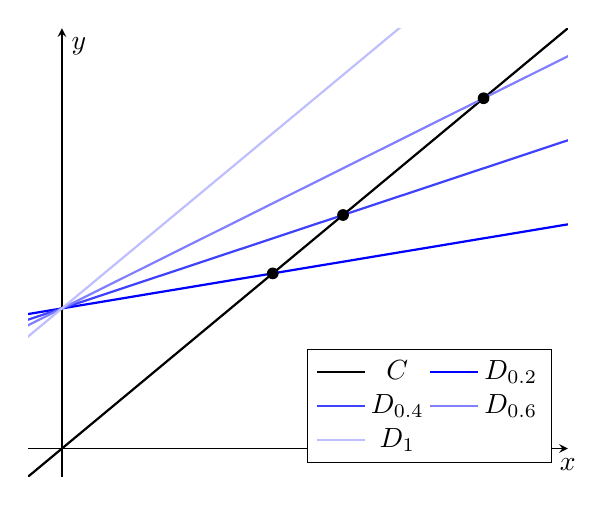
\begin{tikzpicture}
\begin{axis}[axis lines=middle,xmin=-0.2,xmax=3,ymin=-0.2,ymax=3,xtick=\empty,ytick=\empty,xlabel=$x$,ylabel=$y$,legend pos=south east,xlabel style={anchor=north},legend columns=2]
\addplot[smooth,samples=1000,no markers,thick] {x};
\addplot[smooth,samples=1000,no markers,thick,blue] {0.2*x+1};
\addplot[smooth,samples=1000,no markers,thick,blue!75] {0.4*x+1};
\addplot[smooth,samples=1000,no markers,thick,blue!50] {0.6*x+1};
\addplot[smooth,samples=1000,no markers,thick,blue!25] {x+1};
\node[circle,fill,inner sep=1.5pt] at (5/4,5/4) {};
\node[circle,fill,inner sep=1.5pt] at (5/3,5/3) {};
\node[circle,fill,inner sep=1.5pt] at (5/2,5/2) {};
\legend{$C$,$D_{0.2}$,$D_{0.4}$,$D_{0.6}$,$D_1$};
\end{axis}
\end{tikzpicture}
\end{center}

Usually they have one intersection if $t\neq 1$ as shown above, so the theorem holds. But as $t$ approaches 1, the intersection points goes to infinity, and in the usual sense $C$ and $D_1$ don't intersect. Hence we need to compactify the space from $k^2$ the affine space to $\p^2_k$ the projective space: we identify $(x,y)\in k^2$ with 1-dimensional $k$-linear subspace of $k^3$ spanned by $(x,y,1)$, i.e. define $\p^2_k=k^3\backslash\{0\}/\sim$ where $x\sim y$ if $x=\lambda y$ for some $\lambda\in k^\times$. Then the 1-dimensional subspaces of $\{(x,y,0)\in k^3\}$ (can be thought as forming $\p^1_k$) are ``points at infinity''.
\end{enumerate}

More generally, $\p^n(k):=k^{n+1}\backslash\{0\}/\sim$ are defined similarly and such an equivalence class is denoted by $[x_0,x_1,\cdots,x_n]$. Note that at least one $x_i\neq 0$. One has the embedding $\phi:k^n=\A_k^n\rightarrow\p_k^n:(x_1,\ldots,x_n)\mapsto [1,x_1,\cdots,x_n]$ and so $\p_k^n=\im\phi\cup\p_k^{n-1}$ where $\p_k^{n-1}=\{[0,x_1,\cdots,x_{n }]\}$.

Now consider $\ell:k^{n+1}\rightarrow k:(x_0,\ldots,x_n)\mapsto\alpha_0x_0+\cdots+\alpha_nx_n$ where $\alpha_i\in k$ not all zero. Define the \textit{kernel} of this function in the sense that
\[
\ker\ell=\{[x_0,\cdots,x_n]\in\p_k^n:\alpha_0x_0+\cdots+\alpha_nx_n=0\},
\]
which is a linear hyperplane (in particular a subspace) in $\p_n^k$. More generally,
\begin{defn}
A function $f\in k[x_0,\ldots,x_n]$ is \textit{homogeneous} of degree of $d$ if
\[
f(x_0,\ldots,x_n)=\sum_{i_0+\cdots+i_n=d}\alpha_{i_0\cdots i_n}x_0^{i_0}x_n^{i_n},\quad\text{i.e. there are only degree }d\text{ terms}.
\]
\end{defn}
If $(x_0,\ldots,x_n)$ is a zero point of such $f$ then $(\lambda x_0,\ldots,\lambda x_n)$ is one as well, so the following is well defined:
\[
C_f=\{[x_0,\ldots,x_n]\in\p_k^n:f(x_0,\ldots,x_n)=0\}.
\]

If $f\in k[x_1,\ldots,x_n]$ is not homogeneous, one can \textit{homogenise} it:
\[
\begin{aligned}
&\quad f(x_1,\ldots,x_n)=\sum_{i_1+\cdots+i_n\leq d}\alpha_{i_1\cdots i_n}x_1^{i_1}\cdots x_n^{i_n}\\
&\leadsto f(x_0,x_1,\ldots,x_n)=\sum_{i_0+\cdots+i_n=d}\alpha_{i_1\cdots i_n}x_0^{d-i_1-\cdots-i_n}x_1^{i_1}\cdots x_n^{i_n}.
\end{aligned}
\]

If a $f\in k[x_0,\ldots,x_n]$ is homogeneous, one can \textit{dehomogenise} it by setting one of the variables $x_i$ to 1.

Hence for a general $f(x,y)$, denote the homogenisation of it by $F(X,Y,1)$ (we capitalise to show homogeneity) and define the projective curve
\[
C_f=\{(x,y):f(x,y)=F(X,Y,1)=0\}\subset\A_k^2
\]
and the points at infinity are $[X,Y,0]:F(X,Y,0)=0$, and one can write $C_F=C_f\cup\{\text{points at infinity}\}$ where $\{\text{points at infinity}\}=C_F\cap\p_k^1$.

We have now resolved the four issues and can give a more precise form of what we want to prove.

\begin{thm}[Bézout's, formal statement]
\label{thm:Bezout}
Let $K=\overline k$ and $F,G\in k[X_0,X_1,X_2]$ be nonzero and homogeneous without common factors. Then
\[
\sum_{p\in C_F(K)\cap C_G(K)} (C_F\cdot C_G)_p=\deg F \deg G.
\]
\end{thm}

\begin{flushright}
\textit{Week 3, lecture 3, 18th October}
\end{flushright}

\subsection{More tools for studying projective curves}

\begin{defn}
We say two projective curves are \textit{equivalent} if they are related by a projective linear change of coordinates:
\[
\begin{aligned}
\widetilde X&=c_{11}X+c_{12}Y+c_{13}Z \\
\widetilde Y&=c_{21}X+c_{22}Y+c_{23}Z \\
\widetilde Z&=c_{31}X+c_{32}Y+c_{33}Z
\end{aligned}
\]
where $(c_{ij})$ is an invertible matrix over $K$.
\end{defn}

\begin{defn}
A point $p\in C_F$ on a projective curve is \textit{singular} at $p$ if $F(p)=0$ and $\frac{\partial F}{\partial x}(p)=\frac{\partial F}{\partial y}(p)=\frac{\partial F}{\partial z}(p)=0.$

Define \textit{smooth} similarly.
\end{defn}

See a proof of $p\in C_f$ is singular $\iff p\in C_F$ is singular in Algebraic curves MATH70033, and $k^2$ is bijective with each affine chart $U_1=\{[1,x,y]\},U_2=\{[x,1,y]\},U_3=\{[x,y,1]\}$.

Any conic in $\p_k^2$ (with $\Char k\neq 2$) is given by
\[
Q(X_1,X_2,X_3)=\sum_{i,j=1}^3 q_{ij}X_iX_j\qquad (q_{ij})\text{ is a symmetric }3\times 3\text{ matrix over }k
\]
\begin{remark}
A conic defined as above is smooth $\iff(q_{ij})$ is invertible. Indeed, $Q$ is singular if
\[
\begin{aligned}
\frac{\partial Q}{\partial X_1}&=2(q_{11}X_1+q_{12}X_2+q_{13}X_3) \\
\frac{\partial Q}{\partial X_2}&=2(q_{21}X_1+q_{22}X_2+q_{23}X_3) \\
\frac{\partial Q}{\partial X_3}&=2(q_{31}X_1+q_{32}X_2+q_{33}X_3)
\end{aligned}
\]
has a solution.
\end{remark}

\begin{lemma}
\label{lemma:conicsingulariffreducible}
Let $k$ be a field with $\Char k\neq 2$ and $C_Q\subset\p_k^2$ a conic. Then $C_Q$ is singular $\iff Q$ is a product of linear polynomials $\overline k$.
\end{lemma}
\begin{proof}
\begin{itemize}
\item[$\implies$] Recall from linear algebra that after a linear change of coordinates one can write
\[
Q(X_1,X_2,X_3)=a_1X_1^2+a_2X_2^2+a_3X_3^2
\]
since $Q$ is a quadratic form $k^3\rightarrow k$. Hence by the remark above, $Q$ is singular $\iff a_1a_2a_3=0$. WLOG assume $x_3=0$, then
\[
Q=a_1X_1^2+a_2X_2^2=\left(\sqrt{a_1}X_1+i\sqrt{a_2}X_2\right)\left(\sqrt{a_1}X_1-i\sqrt{a_2}X_2\right).
\]
\item[$\impliedby$] Write $Q=L_1L_2$ where $L_i\in\overline k[X_1,X_2,X_3]$ are linear. If $L_1=L_2$ then again after a linear change of coordinates one can write $L_1=L_2=X_1$, so $Q=X_1^2$ and hence $\det q_{ij}=0$. If $L_1\neq L_2$ then by \ref{thm:Bezout} $\exists P\in L_1\cap L_2$, and
\[
\frac{\partial Q}{\partial X_i}(P)=\frac{\partial L_1}{\partial X_i}(P)L_2(P)+\frac{\partial L_2}{\partial X_i}(P)L_1(P)=0,
\]
so $Q$ is singular at $P$.
\end{itemize}
\end{proof}

\begin{example}
Higher degrees are not so easy. $F=Y^2Z-X^3$ defines $C_F\subset\p^2$ and
\[
\begin{aligned}
\frac{\partial F}{\partial X}(0,0,1)=3\cdot 0^2&=0 \\
\frac{\partial F}{\partial Y}(0,0,1)=2\cdot 1\cdot 0&=0\\
\frac{\partial F}{\partial Z}(0,0,1)=-0^2&=0,
\end{aligned}
\]
but $Y^2Z-X^3$ is irreducible.
\end{example}

\begin{prop}
\label{prop:flexHessian}
Let $F\in k[X_1,X_2,X_3]$ with $\deg F=d$ and $C_F\subset\p_k^2$ be smooth. If $\Char k\nmid 2(d-1)$, then $P\in C_F$ is flex $\iff H(P)=0$ where
\[
H(X_1,X_2,X_3)=\det\left(\frac{\partial^2 F}{\partial X_i\partial X_j}\right)_{1\leq i,j\leq 3} \qquad\text{(the Hessian)}
\]
\end{prop}

\begin{center}
\begin{tikzpicture}
\begin{axis}[axis lines=middle,xmin=-2.5,xmax=1.5,ymin=-1.5,ymax=2.5,xtick=\empty,ytick=\empty,xlabel=$x$,ylabel=$y$,legend pos=north west,xlabel style={anchor=north}]
\addplot[thick,smooth] table {data2.dat};
\addplot[no markers,thick,blue] {x+2};
\addplot[thick,smooth,blue!25] table {data3.dat};
\node[circle,fill,inner sep=1.5pt,label={180:{$P$}}] at (-1,1) {};
\legend{$C$,$L$,$Q$};
\end{axis}
\end{tikzpicture}
\end{center}

\begin{proof}
Write $P=(P_1,P_2,P_3)$. Since $F(P)=0$ one can write
\[
F(P_1+X_1,P_2+X_2,P_3+X_3)=\underbrace{\sum_{i=1}^3\frac{\partial F}{\partial X_i}(P)X_i}_{\text{tangent line }L}+\underbrace{\frac12\sum_{i,j=1}^3\frac{\partial^2 F}{\partial X_i\partial X_j}(P)X_iX_j}_{\text{osculating conic }Q}+\cdots
\]
Recall from Algebraic curves a result due to Euler:
\[
\sum_{i=1}^3 X_i\frac{\partial F}{\partial X_i}=dF.
\]
Differentiating the above one has
\[
\sum_{i,j=1}^3X_iX_j\frac{\partial^2 F}{\partial X_i\partial X_j}=d(d-1)F=Q,
\]
so $P\in Q$. Now the tangent line to $Q$ at $P$ is
\[
2\sum_{i=1}^3\left(\sum_{j=1}^3\frac{\partial^2 F}{\partial X_i\partial X_j}(P)P_j\right)X_i=2(d-1)\sum_{i=1}^3\frac{\partial F}{\partial X_i}(P)X_i=0,
\]
so it's the same line with $L$ when $2(d-1)\neq 0$. Hence since $C_F$ is smooth, $Q$ is smooth at $P$.

\begin{flushright}
\textit{Week 4, lecture 1, 22nd October}
\end{flushright}

Note that $P$ is flex $\iff L\subset Q$: the $\impliedby$ is clear, and the $\implies$ follows from the way we count multiplicities. Hence by \ref{lemma:conicsingulariffreducible} $Q\supset L$ is not smooth by and singular at some point $S=(S_1,S_2,S_3)$. Then $H(P)\begin{pmatrix}S_1 & S_2 & S_3\end{pmatrix}^T=0$, hence $H(P)=0$.
\end{proof}

\begin{example}
\label{example:Hessianflex}
Consider $C=\{F=X^3+Y^3+Z^3+3XYZ=0\}$, then
\[
\begin{aligned}
\frac{\partial F}{\partial X}&=3X^2+3YZ \\
\frac{\partial F}{\partial Y}&=3Y^2+3XZ \\
\frac{\partial F}{\partial Z}&=3Z^2+3XY
\end{aligned}
\]
so
\[
\det H_F=\begin{pmatrix}
6X & 3Z & 3Y \\ 3Z & 6Y & 3X \\ 3Y & 3X & 6Z
\end{pmatrix}=-54 (x^3 + y^3 - 5xyz + z^3)
\]
which is another cubic, so the flex points by above are simply intersections of these cubics.

\begin{center}
\begin{tikzpicture}
\begin{axis}[axis lines=middle,xmin=-2,xmax=2.5,ymin=-2,ymax=2,xtick=\empty,ytick=\empty,xlabel=$x$,ylabel=$y$,legend pos=south east,xlabel style={anchor=north}]
\addplot[thick,smooth] table {data4.dat};
\addplot[thick,blue,smooth] table {data5.dat};
\addplot[thick,no marks,smooth,domain=-2:2.2,blue!50] {x-1};
\addplot[thick,no marks,smooth,domain=-0.3:2.2] {1};
\node[circle,fill,inner sep=1.5pt,label={180:{$P=[0,-1,1]$}}] at (0,-1) {};
\node[circle,fill,inner sep=1.5pt,label={270:{$S$}}] at (2,1) {};
\legend{$C_F$,$C_{\det H_F}$,$L$};
\end{axis}
\end{tikzpicture}
\end{center}

One has
\[
H_F(0,-1,1)=\begin{pmatrix}0 & 3 & -3 \\ 3 & -6 & 0 \\ -3 & 0 & 6\end{pmatrix}.
\]

Now the tangent line at $[0,-1,1]$ is
\[
L=\left\{\frac{\partial F}{\partial X}(0,-1,1)X+\frac{\partial F}{\partial Y}(0,-1,1)Y+\frac{\partial F}{\partial Z}(0,-1,1)Z=-3X+3Y+3Z=0\right\}=\{X-Y-Z=0\}
\]
and the osculating conic is
\[
\begin{aligned}
Q&=\{3XY-3XZ+3XY-6Y^2-3XZ+6Z^2=0\}=\{XY-XZ-Y^2+Z^2=0\}\\&=\{(X-Y-Z)(Y-Z)=0\}=\{X-Y-Z=0\}\cup\{Y-Z=0\}.
\end{aligned}
\]
\end{example}

\begin{coro}
\label{coro:Weierstrassform}
Let $C\subset\p^2_k$ be a smooth projective cubic curve with $k$ algebraically closed and $\Char k\neq 2$. Then $\exists$ a projective linear change of coordinates such that the equation of $C$ takes the Weierstrass form
\[
Y^2Z=X^3+a_2X^2Z+a_4XZ^2+a_6Z^3
\]
\[
(\text{the affine form is then }y^2=f(x)=x^3+a_2x^2+a_4x+a_6\text{ which has distinct roots})
\]
\end{coro}
\begin{proof}
Since $k$ is algebraically closed, by the observation above and \ref{thm:Bezout}, $C=\{F(X,Y,Z)=0\}\subset\p^2$ has exactly 9 flex points, so let $P\in C$ be flex. Choose a linear change of coordinates such that $P=[0,1,0]$ and tangent at $P$ is $\{Z=0\}$. Parametrise the tangent line by $F(t,1,0)$, then since $P$ is flex, the tangent must vanish to order 3, so $F(t,1,0)=ct^3 (\ast)$ for some $c\in k$. But then one can write
\[
F(X,Y,Z)=\alpha Y^2Z+a_1XYZ+a_3YZ^2-\beta X^3-a_2X^2Z-a_4XZ^2-a_6Z^3
\]
since it cannot have $X^2Y,XY^2$ or $Y^3$ terms by $\ast$. Now $C$ is smooth, so $P$ is not singular, but
\[
\begin{aligned}
\frac{\partial F}{\partial X}(0,1,0)&=a_1YZ-3\beta X^2-2a_2ZX-a_4Z^2=0 \\
\frac{\partial F}{\partial Y}(0,1,0)&=2\alpha ZY+a_1XZ+a_3Z^2=0
\end{aligned}
\]
hence
\[
\frac{\partial F}{\partial Z}(0,1,0)=\alpha Y^2+a_1 XY+2a_3YZ-a_2X^2-2a_4XZ-3a_6Z^3=\alpha\neq 0
\]
and $\beta\neq 0$ again by $\ast$, so one can rescale by $X\mapsto \alpha\beta X,\ Y\mapsto\alpha\beta^2Y$ and write
\[
Y^2Z+a_1XYZ+a_3YZ^2=X^3+a_2X^2Z+a_4XZ^2+a_6Z^3,
\]
and finally by $Y\mapsto Y-\frac{a_1}{2}X-\frac{a_3}{2}Z$ (note that this doesn't disturb $P$) one has
\[
Y^2Z=X^3+a_2X^2Z+a_4XZ^2+a_6Z^3,
\]
the desired form. $f(x)$ has no repeated roots since $C$ is smooth.
\end{proof}

\begin{remark}
If $\Char k=2$, then $\exists$ a Weierstrass form
\[
y^2+a_1xy+a_3y=x^3+a_2x^2+a_4x+a_6,
\]
in particular we can't divide by two so we couldn't do the last step in the proof above.
\end{remark}

\section{Conics: Hasse--Minkowski theorem}

\begin{thm}[Hasse--Minkowski]
\label{thm:HasseMinkowski}
Let $C\subset\p_\Q^2$ be a curve defined by $Q=aX^2+bY^2+cZ^2$ where $a,b,c\in\Z$ are squarefree such that $abc\neq 0,\ (a,b)=(b,c)=(a,c)=1$. Then the following are equivalent:
\begin{enumerate}
\item $Q$ has infinitely many solutions in $\p_\Q^2$.
\item $Q$ has a solution in $\p_\Q^2$.
\item $Q$ has a solution in $\p_{\Q_p}^2 \ \forall p$ and in $\p_\R^2$.
\item $Q$ has a solution in $\p_{\Q_p}^2 \ \forall p\in\Sigma:=\{p:p\mid 2abc\}$.
\end{enumerate}
\end{thm}

Trivially $1\implies 2\implies 3\implies 4$, so it suffices to show $3\implies 2$, $4\implies 2$ and $2\implies 1$.

\begin{flushright}
\textit{Week 4, lecture 2, 24th October}
\end{flushright}

\subsection{Proof of $3\implies 2$}

\begin{prop}
If $Q$ is the conic given by $aX^2+bY^2+cZ^2=0$ (this is the general form by diagonalising the quadratic form) over $\Q_p$ with $p\nmid 2abc$, then it always have a solution.
\end{prop}
\begin{proof}
One can assume $a,b,c\in\Z_p$ since the conic is invariant up to rescaling. Since $p\nmid 2abc$, one has $|a|_p=|b|_p=|c|_p=1$. If $Q$ has a solution in $\Q_p$ then it better had a solution in $\F_p$, so reduce mod $p$ and fix $x\in\F_p$. Define
\[
A:=\{ax^2+by^2:y\in\F_p\},\quad B:=\{-cz^2:z\in\F_p\},
\]
then solutions over $\F_p$ are precisely $A\cap B$. We claim $|A|=|B|=\frac{p+1}{2}$. Indeed, consider the map $\F_p\rightarrow\F_p:y\mapsto ax^2+by^2$. It's not injective: if $ax^2+by_1^2=ax^2=by_2^2$ then $by_1^2=by_2^2$, but $b$ is a unit (since $p\nmid b$) so $y_1^2=y_2^2$, i.e. $y_1=\pm y_2$, hence $|A|=1+\frac{p-1}{2}=\frac{p+1}{2}$ (since $0=-0$). The argument for $|B$| is similar. Then $|A|+|B|=p+1>p$, so by pigeonhole $A\cap B\neq\varnothing$. Let $(x_0,y_0,z_0)$ be a solution over $\F_p$ with $x_0\neq 0$ and consider $f(x)=ax^2+by_0^2+cz_0^2\in\Z_p[x]$ with $x_0$ as a solution. One has $f'(x_0)=2ax_0\neq 0$, so by \ref{lemma:Hensel} we can lift to a solution in $\Q_p$.
\end{proof}

\begin{remark}
Having dealt with large primes, let's deal with reals. Let $aX^2+bY^2+cZ^2=0$ be over $\R$. Note that one can rewrite the equation as $(\sqrt a X)^2+(\sqrt b Y)^2+(\sqrt c Z^2)=0$ so assume WLOG $a,b,c\in\{\pm 1\}$. But $X^2+Y^2+Z^2=0$ has no solutions so consider $X^2+Y^2-Z^2=0$ (which is the same equation as $X^2-Y^2+Z^2,X^2-Y^2-Z^2$, etc. since they are simply scalar multiples of each other), which clearly has solutions over $\R$.
\end{remark}

\begin{remark}
Now consider primes $p:p\mid 2abc$ and how one might obtain solutions over $\Q$ from $\Q_p$. Let $aX^2+bY^2+cZ^2=0$ be over $\Q$ with $a,b,c\in\Q$. WLOG one can assume
\begin{enumerate}
\item $a,b,c\in\Z$ (just multiply by common denominators),
\item $a,b,c$ are coprime (rescaling by common divisor),
\item $a,b,c$ are square free (absorb squares into $X,Y,Z$) and
\item $a,b,c$ are pairwise coprime (if $p\mid a,p\mid b$ then $p^2\mid pa,p^2\mid pb$ so one can absorb $p^2$ in to $X,Y$ with the cost of multiplying $c$ by $p$ but the total number of $p$'s that divide $a,b,c$ decreases).
\end{enumerate}
Now let $p$ be an odd prime such that $p\mid 2abc$, and WLOG assume $p\mid a$ but $p\nmid b,c$, i.e. $|a|_p=\frac{1}{p}$ and $|b|_p=|c|_p=1$. For $aX^2+bY^2+cZ^2=0$ to have a solution over $\Q$, it's necessary for it to have a solution over $\F_p$, so reduce mod $p$ and consider $bY^2+cZ^2=0$ over $\F_p$. Clearly if this has a solution, then again one can lift it to $\Q_p$ by \ref{lemma:Hensel}.

If $p=2$, it's not enough to reduce $\F_2$ and one has to consider $\F_8$ and use the stronger form of \ref{lemma:Hensel}.

So believing the main theorem, we have an algorithm to solve a general conic over $\Q$.
\end{remark}

\subsection{Proof of $4\implies 2$ by geometry of numbers}
\begin{defn}
For $S\subset\R^n$, define its \textit{volume} by the Lebesgue
\[
\vol(S)=\int_S 1_S(x)\ \mathrm d\mu \qquad \text{where }1_S(x)=\left\{\begin{aligned}
1 \quad x\in S \\
0 \quad x\notin S
\end{aligned} \right.
\]
In this case $S$ is \textit{measurable}.
\end{defn}


\begin{lemma}[Blichfeldt]
\label{lemma:Blichfeldt}
Let $S\subset\R^n$ be measurable with $\vol(S)>m\in\Z_{>0}$. Then there are $m+1$ points in $S$ that have integer vector differences, i.e. $\exists s_0,\ldots,s_m\in S:s_i-s_j\in\Z^n \ \forall 0\leq i,j\leq m$.
\end{lemma}

\begin{center}
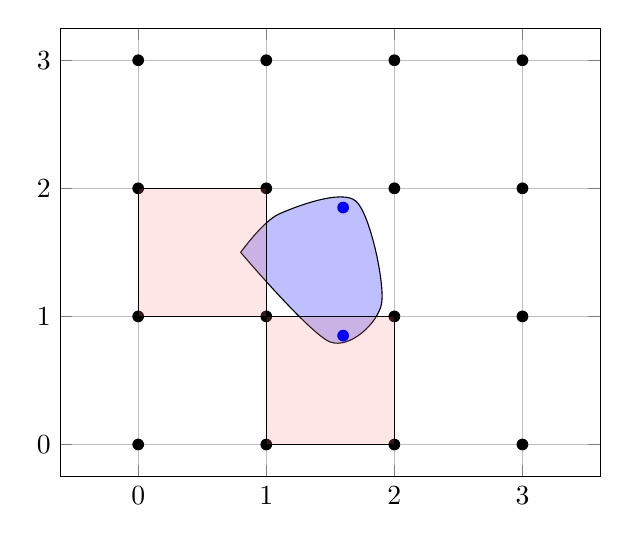
\begin{tikzpicture}
\begin{axis}[xmin=-0.25,xmax=3.25,ymin=-0.25,ymax=3.25,grid=major,axis equal,xtick={0,1,2,3},ytick={0,1,2,3}]
\node[circle,fill,inner sep=1.5pt] at (0,0) {};
\node[circle,fill,inner sep=1.5pt] at (0,1) {};
\node[circle,fill,inner sep=1.5pt] at (0,2) {};
\node[circle,fill,inner sep=1.5pt] at (0,3) {};
\node[circle,fill,inner sep=1.5pt] at (1,0) {};
\node[circle,fill,inner sep=1.5pt] at (1,1) {};
\node[circle,fill,inner sep=1.5pt] at (1,2) {};
\node[circle,fill,inner sep=1.5pt] at (1,3) {};
\node[circle,fill,inner sep=1.5pt] at (2,0) {};
\node[circle,fill,inner sep=1.5pt] at (2,1) {};
\node[circle,fill,inner sep=1.5pt] at (2,2) {};
\node[circle,fill,inner sep=1.5pt] at (2,3) {};
\node[circle,fill,inner sep=1.5pt] at (3,0) {};
\node[circle,fill,inner sep=1.5pt] at (3,1) {};
\node[circle,fill,inner sep=1.5pt] at (3,2) {};
\node[circle,fill,inner sep=1.5pt] at (3,3) {};
\addplot[smooth,fill=blue!25] coordinates {(0.8,1.5) (1.1,1.8) (1.7,1.9) (1.9,1.1) (1.5,0.8) (0.8,1.5)};
\addplot[fill=red!50,fill opacity=0.2] coordinates {(0,1) (1,1) (1,2) (0,2) (0,1)};
\addplot[fill=red!50,fill opacity=0.2] coordinates {(1,0) (2,0) (2,1) (1,1) (1,0)};
\node[circle,fill,inner sep=1.5pt,blue] at (1.6,0.85) {};
\node[circle,fill,inner sep=1.5pt,blue] at (1.6,1.85) {};
\end{axis}
\end{tikzpicture}
\end{center}

Blichfeldt says: an area greater than 1 has 2 points in it that are 1 unit apart. The idea is that one can translate squares which contain pieces of the area (the red ones) around the middle one into the middle so that there must be an overlap.

\begin{proof}
Consider $U:[0,1)\times\cdots[0,1)\subset\R^n$, the standard cube, which has $\vol(U)=1$, and one can tile the whole $\R^n$ with copies of $U$ together with $\Z^n$. Now
\[
\begin{aligned}
m<\vol(S)&=\int_{\R^n}1_S(x)\ \mathrm d\mu \\
&=\sum_{t\in\Z^n}\int_{U+t}1_S(x)\ \mathrm d\mu \qquad \text{by property of Lebesgue integral} \\
&=\sum_{t\in\Z^n}\int_{U}1_S(x+t)\ \mathrm d\mu \qquad \text{translation invariance} \\
&=\int_{U}\sum_{t\in\Z^n}1_S(x+t)\ \mathrm d\mu,
\end{aligned}
\]
in particular $\sum_{t\in\Z^n}1_S(x+t)>m$ at some $x\in U$, otherwise its integral wouldn't $>m$ since $\vol(U)=1$. But this function counts $t$ such that the point $x+t$ is in $S$, i.e. number of points that are integer distance apart.
\end{proof}

\begin{defn}
$S\subset\R^n$ is \textit{symmetric} if $x\in S\implies -x\in S$, is \textit{convex} if $x,y\in S\implies tx+(1-t)y\in S$ for $t\in [0,1]$.
\end{defn}

\begin{coro}[Minskowski's geometry of numbers]
\label{coro:Minkowski}
Let $\Lambda\subset\Z^n$ be a subgroup of finite index $m$ and $C\subset\R^n$ an open, convex, symmetric set such that $\vol(C)>2^nm$. Then $\Lambda\cap C\neq\{0\}$, i.e. there is another nontrivial common point of $\Lambda$ and $C$.
\end{coro}
\begin{proof}
Apply \ref{lemma:Blichfeldt} to $S=\left\{\frac12 x:x\in C\right\}$ with $\vol(S)=2^{-n}\vol C>m$. Now
\[
|\{s_i-s_0:i=0,\ldots,m\}|=m+1>[\Z^n:\Lambda],
\]
so two of them are in the same coset, i.e. $\exists i\neq j:(s_i-s_0)-(s_j-s_0)=s_i-s_j\in\Lambda$. But now $2s_i,-2s_j\in C$ by construction and that $C$ is symmetric, so $s_i-s_j=\frac{2s_i}{2}+\frac{-2s_j}{2}\in C$ since $C$ is convex.
\end{proof}

\begin{flushright}
\textit{Week 4, lecture 3, 25th October}
\end{flushright}

\begin{thm}
If $m\in\Z_{>0}$ satisfies $\exists t:t^2\equiv -1\Mod m$ (i.e. $-1$ is a quadratic residue mod $m$), then $m$ is a sum of two squares.

In particular, any prime $p\equiv 1\Mod 4$ is a sum of two squares.
\end{thm}
\begin{proof}
Let $\Lambda=\{(x,y):y\equiv tx\Mod m\}$. To see this is a subgroup of $\Z^2$ of index $m$, note that it's precisely $\ker\varphi$ where $\varphi:\Z^2\rightarrow\Z/m:(x,y)\mapsto y-tx$. Let $C=\{(x,y)\in\R^2:x^2+y^2<2m\}$, an open ball and clearly convex and symmetric with $\vol(C)=2m\pi>2^2m$, so one has $0\neq (x,y)\in\Lambda \cap C$. In particular, $x^2+y^2<2m$ and $y\equiv tx\Mod m$, so
\[
x^2+y^2\equiv x^2+t^2x^2=(t^2+1)x^2\equiv 0\Mod m,
\]
hence $m=x^2+y^2$.
\end{proof}

\begin{prop}
With the same setup as \ref{thm:HasseMinkowski}, if $Q$ has a solution over $\Q_p$ for all $p\in\Sigma$ then it has a solution over $\Q$.
\end{prop}
\begin{proof}
If we can construct a subgroup $\Lambda\subset\Z^3$ of index $4|abc|$ with $Q(x,y,z)\equiv 0\Mod 4|abc| \ \forall (x,y,z)\in\Lambda$, then $C=\{|a|X^2+|b|Y^2+|c|Z^2<4|abc|\}$ is an open ellipsoid which is convex and symmetric with
\[
\vol(C)=\frac{\frac43\pi\sqrt{|4abc|^3}}{\sqrt{|abc|}}>2^3|4abc|,
\]
so by \ref{coro:Minkowski} one has $0\neq (r,s,t)\in\Lambda\cap C$, in particular $r,s,t\in\Z,\ ar^2+bs^2+ct^2\equiv 0\Mod 4|abc|$ and $ar^2+bs^2+ct^2<4|abc|$, hence $ar^2+bs^2+ct^2=0$.

So it remains to construct this $\Lambda=\{(r,s,t)\in\Z^3\}$.

If $p\neq 2$, suppose $p\mid a$ (and for $p\mid b,p\mid c$ the argument is symmetric). Note that $\exists r_p\in\Z/p\Z:b+cr_p^2\equiv 0\Mod p$. Indeed, the assumption says $\exists x,y,z\in\Q_p:ax^2+by^2+cz^2=0$, but one can assume $x,y,z\in\Z_p$ not all divisible by $p$ by clearing denominators and divide all by $p$ enough times. If $p\mid y$ then $cz^2=-ax^2-by^2\equiv 0\Mod p$, so $p\mid z$ since $a,b,c$ coprime, $p\mid a \implies p\nmid c$ and hence $p\mid x$, a contradiction. Hence $|y|_p=1$, i.e. $y\in\Z_p^\ast$, so write
\[
a\left(\frac{x}{y}\right)^2+b+c\left(\frac{z}{y}\right)^2=0,\quad \frac{x}{y},\frac{z}{y}\in\Z_p \leadsto b+c\left(\frac{z}{y}\right)^2\equiv 0\Mod p
\]
as desired. Now we claim $\{(r_p,s,t):r_ps+t\equiv 0\Mod p\}$ satisfies the desired congruence property of $\Lambda$. Indeed,
\[
ar_p^2+bs^2+ct^2\equiv bs^2+ct^2\equiv bs^2+cr_p^2s^2=s^2(b+cr_p^2)\equiv 0\Mod p \quad \text{(in particular mod }4|abc|\text{)}
\]

If $p=2$, suppose $2\mid a$ (and for $b,c$ the argument is symmetric). If one can find $(r,s,t):ar^2+bs^2+ct^2\equiv 0\Mod 8$ then the congruence property is satisfied. By a similar argument to above, $\exists x,y,z\in\Z_2:|x|_2\leq 1,|y|_2=|z|_2=1$ and $ax^2+by^2+cz^2=0$, then $0=ax^2+by^2+cz^2\equiv ax^2+b+c\Mod 8$ since any odd number $2n+1$ squares to $4n^2+4n+1=4n(n+1)+1\equiv 1\Mod 8$ (either $n$ or $n+1$ is even).
\begin{itemize}
\item If $x$ is odd then $a+b+c\equiv 0\Mod 8$, and we claim $\{(r,s,t):s\equiv t\Mod 4,\ r\equiv s\Mod 2\}$ satisfies the desired congruence property of $\Lambda$. Indeed, by this condition either $r,s,t$ are all odd, then $ar^2+bs^2+ct^2\equiv a+b+c\equiv 0\Mod 8$, or $r,s,t$ are all even, then $ar^2+bs^2+ct^2\equiv bs^2+ct^2\equiv 4(b+c)\equiv -4a\equiv 0\Mod 8$.
\item If $x$ is even then $b+c\equiv 0\Mod 8$, and we claim $\{(r,s,t):s\equiv t\Mod 4,\ r\equiv 0\Mod 2\}$ satisfies the desired congruence property of $\Lambda$. Indeed, $ar^2+bs^2+ct^2\equiv bs^2+ct^2\equiv (b+c)s^2\equiv 0\Mod 8$.
\end{itemize}
If $p=2\nmid abc$ then $a,b,c$ are odd and assume $(x,y,z)\in\Z_2:ax^2+by^2+cz^2=0$ with $\max(|x|_2,|y|_2,|z|_2)=1$ (i.e. $x,y,z$ not all divisible by 2). Then $ax^2+by^2+cz^2\equiv x^2+y^2+z^2 \equiv 0\Mod 2$, so WLOG $x$ is even and $y,z$ are odd. Then $0\equiv ax^2+by^2+cz^2\equiv by^2+cz^2\equiv b+c\Mod 4$. We claim $\{(r,s,t):r\equiv 0\Mod 2,\ s\equiv t\Mod 2\}$ satisfies the desired congruence property of $\Lambda$. Indeed, $ar^2+bs^2+ct^2\equiv bs^2+ct^2\equiv (b+c)s^2\equiv 0\Mod 4$.

Now let $\Lambda$ be the union of all above sets $\{(r,s,t)\in\Z^3\}$ which has index $|4abc|$ by Chinese remainder theorem, and we have checked case by case that $ar^2+bs^2+ct^2\equiv 0\Mod 4abc \ \forall (r,s,t)\in\Lambda$.
\end{proof}

\begin{flushright}
\textit{Week 5, lecture 1, 29th October}
\end{flushright}

To prove \ref{thm:HasseMinkowski}, it now remains to show $2\implies 1$. Before that let's do an example believing the theorem is true.
\begin{example}
Does $F(X,Y,Z)=7X^2+3Y^2-2Z^2+4YZ+6XZ+2XY$ have a rational solution? The first thing is to diagonalise (by $Y\mapsto Y-\frac{4X}{5},Z\mapsto Z+Y+\frac{7X}{10}$) to $\frac{1}{10}(83X^2+50Y^2-20Z^2)$ and we can make the coefficients integers and squarefree and simply consider $83X^2+2Y^2-5Z^2=0$. Then we only have to check if it has solutions over $\Q_p$ where $p\mid 1660=2^2\times 5\times 83$, so $\Q_2,\Q_5$ and $\Q_{83}$.

In $\Q_5$ one has $83+2\equiv 0\Mod 5$ and in $\Q_{83}$ we have $2\times 8^2-5\times 3^2=83\equiv 0\Mod 83$. In $\Q_2$, recall that it's not enough to reduce mod 2 since the powers come down when taking derivative and Hensel's doesn't work, so we reduce mod 8 and $83+2-5\equiv 0\Mod 8$. So the answer is yes.

Remember these local solutions are not necessarily reductions of global solutions and are simply filters. But once we know it has a global solution we can use geometry of numbers to construct it.
\end{example}

\subsection{Proof of $2\implies 1$}
\begin{prop}
Let $k$ be a field with $\Char k\neq 2$ and $Q$ a conic. If $O\in Q$ is a point over $k$, then one can construct a bijection between points over $k$ of $Q$ and $\p_k^1$, in particular if $Q$ has one point over $k$ it has infinitely many points over $k$.
\end{prop}
We almost saw the proof during the very first lecture: recall how we construct infinitely many rational points on the unit circle in \ref{example:acircletobeginwith}.

\begin{center}
\begin{tikzpicture}
\begin{axis}[axis equal,axis lines=middle,xmin=-3.3,xmax=0.3,ymin=-1.2,ymax=1.2,xtick=\empty,ytick=\empty]
\addplot[thick,smooth] table {data6.dat};
\addplot[no markers,smooth,thick,domain=-3:0.2] {0.4*x+0.7};
\addplot[no markers,smooth,thick,domain=-3:0.2,blue!75] {-0.8*x};
\addplot[no markers,smooth,thick,domain=-3:0.2,blue!50] {-0.1*x};
\node[circle,fill,inner sep=1.5pt,label={45:{$O$}}] at (0,0) {};
\node[circle,fill,inner sep=1.5pt,label={45:{$P$}}] at (-1.2405,0.99243) {};
\node[circle,fill,inner sep=1.5pt,label={180:{$\pi(P)$}}] at (-7/12,7/15) {};
\node[circle,fill,inner sep=1.5pt,label={15:{$P'$}}] at (-2.773,0.2773) {};
\node[circle,fill,inner sep=1.5pt,label={90:{$\pi(P')$}}] at (-1.4,0.14) {};
\node at (-3.1,-0.6) {$\ell$};
\end{axis}
\end{tikzpicture}
\end{center}

\begin{proof}
It suffices to show that with a line $\ell$ over $k$ not containing $O\in Q$, the map $\pi:Q\rightarrow\ell:P\mapsto\ell\cap\overrightarrow{OP}$ is bijective. By \ref{thm:Bezout} the two lines $\ell$ and $\overrightarrow{OP}$ indeed must intersect, and since they are defined over $k$, $\pi(P)$ is over $k$ as well.
\begin{itemize}
\item $\pi$ is surjective: let $L\in\ell$, then $\overrightarrow{OL}\cap Q\neq\varnothing$ has two solutions over $\overline k$, one of them is $O$. But if a quadratic have a solution over $k$ then it must have another over $k$ as well, since if $f=gh$ with $\deg f=2,\deg g=1$ then $\deg h=1$.
\item $\pi$ is injective: if $\pi(P)=\pi(P')$ then $\overrightarrow{OP}=\overrightarrow{OP'}$, hence $P,P',O\in\overrightarrow{OP}\cap Q$, but \ref{thm:Bezout} tells us $|\overrightarrow{OP}\cap Q|=2$ and $P,P'\neq O$ so $P=P'$.
\end{itemize}
\end{proof}

\section{Cubics}
\begin{defn}
A \textit{plane cubic} is an equation $F(X,Y,Z)=0$ where $F\in k[X,Y,Z]$ is homogeneous of degree 3.
\end{defn}

\begin{example}
Two types of singular points of cubics are \textit{cusp} and \textit{node}. Also, the $k$-points of cubic curves can be parametrised, for example the two below: $t\mapsto (t^2,t^3,1)$ and $t\mapsto (t^3-t,t^2-1,1)$ respectively.
\end{example}

\begin{center}
\begin{minipage}{0.4\textwidth}
\begin{center}
\begin{tikzpicture}[scale=0.6]
\begin{axis}[axis equal,axis lines=middle,xmin=-0.1,xmax=1,ymin=-1,ymax=1,xtick=\empty,ytick=\empty]
\addplot[no markers,smooth,thick,samples=1000] {sqrt(x^3)};
\addplot[no markers,smooth,thick,samples=1000] {-sqrt(x^3)};
\end{axis}
\end{tikzpicture}

$Y^2Z=X^3$
\end{center}
\end{minipage}
\begin{minipage}{0.4\textwidth}
\begin{center}
\begin{tikzpicture}[scale=0.6]
\begin{axis}[axis equal,axis lines=middle,xmin=-0.7,xmax=1.5,ymin=-1.5,ymax=1.5,xtick=\empty,ytick=\empty]
\addplot[thick,smooth] table {data7.dat};
\end{axis}
\end{tikzpicture}

$Y^2Z=X^3+X^2Z$
\end{center}
\end{minipage}
\end{center}

\begin{prop}
If $C$ is an irreducible, singular plane cubic over $k$, then $\exists!$ singular $k$-point $p\in C$ such that $C$ has a parametrisation given by lines through $p$.
\end{prop}
\begin{proof}
Suppose $p,q\in C$ are distinct singular points, then the line $L=\overline{PQ}$ intersect $C$ with $(L\cdot C)_p\geq 2,(L\cdot C)_q\geq 2$, a contradiction to \ref{thm:Bezout} since $\deg C=3$.

Now suppose this unique singular point $p$ is over $\overline k$ but not over $k$. Then the Galois group of the extension is not trivial and some $k$-linear automorphism moves it to another singular point (since coefficients of $C$ are in $k$, they don't change), a contradiction.

Finally, the proof for existence of parametrisation is verbatim with the conic case.
\end{proof}

We now move out attention to smooth curves. It's possible that a smooth cubic doesn't have rational points, e.g. $X^3+pY^3+p^2Z^3=0$. It's smooth since the only way that partial derivatives are all zero is that $X=Y=Z=0$, which is not a point in the projective space. Suppose there is a rational point and scale it to coprime integers $a,b,c\in\Z$. Then $a^3=-pb^3-p^2c^3$, so $p\mid a$, hence $p^3\mid pb^3+p^2c^3$. In particular $p^2\mid pb^3$ so $p\mid b$, but then $p^3\mid p^2c$ so $p\mid c$, contradicting $(a,b,c)=1$. So we want to classify smooth cubics with a rational point, which brings us finally to the title of the module.

\begin{defn}
An \textit{elliptic curve} $E$ is a smooth plane cubic over $k$ with a specified $O\in E$ over $k$.
\end{defn}

\subsection{Chord and tangent processes}
\begin{remark}
Recall \ref{example:CTP1stencounter}.

Let $E$ be a cubic with rational points $p,q\in E$. By \ref{thm:Bezout}, the line $\ell_{p,q}$ intersects with $E$ at a third point. But similar to quadratics, if a cubic has two rational solutions, the third one must be rational as well.

In particular, if $p$ is smooth, then the tangent intersects $E$ at another rational point. This is wonderful because it sounds like we can keep generating rational points on a cubic using the so-called \textit{chord and tangent process}: take a smooth rational point and find another one like above, and keep doing this. Now that you have many points, connect them and find even more points.
\end{remark}

\begin{defn}
A rational $p\in E$ is \textit{exceptional} if by chord and tangent process one can only get finitely many points of $E$.
\end{defn}

\begin{flushright}
\textit{Week 5, lecture 2, 31st October}
\end{flushright}

\begin{prop}
Consider the elliptic curve $E:X^3+Y^3=aZ^3$.

If $a>2$ is cubefree, the only exceptional point of $E$ is $[1,-1,0]$.

If $a=1$, the only exceptional points of $E$ are $[1,-1,0],[0,1,1]$ and $[1,0,1]$.

If $a=2$, the only exceptional points of $E$ are $[1,-1,0]$ and $[1,1,1]$.

In particular, any other rational point can be used to find infinitely many rational solutions.
\end{prop}
\begin{proof}
By \ref{prop:flexHessian}, all these points except $[1,1,1]$ are (the only) flex points of $E$. Hence they are exceptional, since the tangent line by definition already intersects with the curve with multiplicity at least 3, so they cannot generate any new point by \ref{thm:Bezout}.

The point $[1,1,1]$ on $X^3+Y^3=2Z^3$ is not flex. But its tangent line $X+Y=2Z$ intersects with the curve at $[1,-1,0]$, which is flex.

Now fix $a\geq 1$ and suppose $\mathbf{x_0}=[x_0,y_0,z_0]\in E$ is an arbitrary other rational point. The tangent line is $\ell_{\mathbf{x_0}}=x_0^2+y_0^2Y-az_0^2Z=0$, which by above intersects $E$ at another point which we claim to be
\[
\mathbf{x_1}=[x_1,y_1,z_1]=[x_0(x_0^3+2y_0^3),-y_0(2x_0^3+y_0^3),z_0(x_0^3-y_0^3)].
\]
One can verify $\mathbf(x_1)\in\ell_{\mathbf{x_0}}\cap E$ simply by substituting. To show that $\mathbf{x_0}$ is not exceptional, by induction it suffices to show $\mathbf{x_1}$ is \textit{higher} than $\mathbf{x_0}$, i.e. after making sure $x_i,y_i,z_i\in\Z$ and $\gcd(x_0,y_0,z_0)=\gcd(x_1,y_1,z_1)=1$ one has $|z_1|>|z_0|$.

Suppose $\gcd(x_0,y_0,z_0)=1$ and let $d=\gcd(x_0(x_0^3+2y_0^3),-y_0(2x_0^3+y_0^3),z_0(x_0^3-y_0^3))$. For any prime $p\mid d$, we claim it's impossible that $p\mid x_0$. Indeed, if so then $p\mid 2y_0x_0^3+y_0^4$ so $p\mid y_0$, but then $az_0^3=x_0^3+y_0^3$ and $a$ is cubefree, so $p\mid z_0$, contradicting $\gcd(x_0,y_0,z_0)=1$. Hence $\gcd(d,x_0)=1$ and symmetrically $\gcd(d,y_0)=\gcd(d,z_0)=1$. So
\[
d\mid (x_0^3+2y_0^3)-2(2x_0^3+y_0^3)=-3x_0^3\quad\text{and}\quad d\mid 2(x_0^3+2y_0^3)-(2x_0^3+y_0^3)=3y_0^3\implies d\mid 3,
\]
hence $d$ is at most 3. It then suffices to show
\[
|z_0||x_0^3-y_0^3|>3|z_0|,\text{i.e. }|x_0^3-y_0^3|>3,
\]
which is true since the only case that $|x_0^3-y_0^3|\leq 3$ is that $x_0,y_0\in\{0,\pm 1\}$, which are flex points.
\end{proof}

\subsection{Group law}
\begin{lemma}[Cayley--Bacharach]
Given 8 points in general position (in particular no 4 are collinear and no 7 lie on the same conic), $\exists$ a 9th point such that any cubic passing through the 8 points must also passes through the 9th.
\end{lemma}

\begin{minipage}{0.4\textwidth}
\begin{center}
\begin{tikzpicture}
\begin{axis}[axis line style={draw=none},xmin=-4,xmax=4,ymin=-4,ymax=4,xtick=\empty,ytick=\empty]
\addplot[thick,smooth,black!50] table {data8.dat};
\addplot[thick,smooth,blue!50] table {data9.dat};
\node[circle,fill,inner sep=1.5pt] at (0,0) {};
\node[circle,fill,inner sep=1.5pt] at (-1.732,1.732) {};
\node[circle,fill,inner sep=1.5pt] at (1.732,-1.732) {};
\node[circle,fill,inner sep=1.5pt] at (-2.236,-2.236) {};
\node[circle,fill,inner sep=1.5pt,blue] at (2.236,2.236) {};
\node[circle,fill,inner sep=1.5pt] at (-0.517638,1.93185) {};
\node[circle,fill,inner sep=1.5pt] at (0.517638,-1.93185) {};
\node[circle,fill,inner sep=1.5pt] at (-1.93185,0.517638) {};
\node[circle,fill,inner sep=1.5pt] at (1.93185,-0.517638) {};
\end{axis}
\end{tikzpicture}
\end{center}
\end{minipage}
\begin{minipage}{0.6\textwidth}
\begin{proof}
Let
\[
g=\sum_{i=0}^{3}a_i X^{3-i}Z^i + \sum_{i=1}^{3}b_i Y^{3-i}Z^i + \sum_{i=1}^2 c_i X^{2-i}Y^i + dXYZ
\]
be a general homogeneous cubic we want to solve for. From the eight points that lie on $E_g$, one has eight linear equations, which are linearly independent by the genral position assumption, leaving 2 degrees of freedom, i.e. $g$ is of the form $\lambda_1f_1+\lambda_2f_2:\lambda_1,\lambda_2\in k$. Then by \ref{thm:Bezout}, $f_1$ and $f_2$ intersect at $3^2=9$ points.
\end{proof}
\end{minipage}

\begin{thm}
Let $E_f$ be an irreducible cubic defined by $f$ over $k$. Suppose $\exists$ at least one $k$-solution $O\in E$. Let $E(k)$ be the set of smooth $k$-points of $E$. Then $E(k)$ has a structure of an abelian group with $O$ as the identity.
\end{thm}

\begin{center}
\begin{tikzpicture}
\begin{axis}[axis line style={draw=none},xmin=-4,xmax=4,ymin=-4,ymax=4,xtick=\empty,ytick=\empty]
\addplot[thick,smooth,black] table {data8.dat};
\addplot[thick,smooth,no markers,samples=1000] {0.164572*x+2.01704};
\addplot[thick,smooth,no markers,samples=1000] {1.03068*x+0.0685899};
\node[circle,fill,inner sep=1.5pt,label={180:{$O$}}] at (-2.236,-2.236) {};
\node[circle,fill,inner sep=1.5pt,label={135:{$P$}}] at (-1.732,1.732) {};
\node[circle,fill,inner sep=1.5pt,label={45:{$Q$}}] at (-0.517638,1.93185) {};
\node[circle,fill,inner sep=1.5pt,label={135:{$R$}}] at (2.2497,2.3873) {};
\node[circle,fill,inner sep=1.5pt,label={180:{$P+Q$}}] at (-0.0136348,0.0545368) {};
\end{axis}
\end{tikzpicture}
\end{center}

\begin{proof}
Define addition on $E(k)$ by: for $P,Q\in E(k)$, take the intersection $R$ of $\overrightarrow{PQ}$ (if $P=Q$, take the tangent line at $P$) and $E_f$, and let $P+Q$ be the third intersection of $\overrightarrow{OR}$ (if $R=O$, take the tangent line at $O$) and $E_f$.

Clearly $P+Q\in E(k)$ again by the fact that the third root of a rational cubic with two known rational solutions must be rational, and if it's singular it contradicts \ref{thm:Bezout}.

\begin{flushright}
\textit{Week 5, lecture 3, 1st November}
\end{flushright}

Now $P+Q=Q+P \ \forall P,Q\in E(k)$ since in the definition we never used the order of $P$ and $Q$, and it's clear that $P+O=P$ ($P$ is the third intersection of the line $\overrightarrow{OR}$ with $E$ where $R\in\overrightarrow{OP}$).

To find $-P$, note that if one draws the tangent line at $O$ which intersects $E$ at $Q$, and the third intersection of $\overrightarrow{QP}$ is $-P$, which is clear from this:

\begin{center}
\begin{tikzpicture}
\begin{axis}[axis line style={draw=none},xmin=-4,xmax=4,ymin=-4,ymax=4,xtick=\empty,ytick=\empty]
\addplot[thick,smooth,black] table {data8.dat};
\addplot[thick,smooth,no markers,samples=1000] {3.04175-0.0325*x};
\addplot[thick,smooth,no markers,samples=1000] {0.69*x+1.38};
\node[circle,fill,inner sep=1.5pt,label={90:{$O$}}] at (-1.15,3.079125) {};
\node[circle,fill,inner sep=1.5pt,label={180:{$P$}}] at (-2,0) {};
\node[circle,fill,inner sep=1.5pt,label={135:{$Q$}}] at (2.3,2.967) {};
\node[circle,fill,inner sep=1.5pt,label={0:{$-P$}}] at (-0.3,1.173) {};
\end{axis}
\end{tikzpicture}
\end{center}

It remains to show associativity, i.e. $\forall P,Q,R\in E(k),\ (P+Q)+R=P+(Q+R)$.

\begin{center}
\begin{tikzpicture}
\begin{axis}[axis line style={draw=none},xmin=-4,xmax=4,ymin=-4,ymax=4,xtick=\empty,ytick=\empty]
\addplot[thick,smooth,black] table {data8.dat};
\addplot[thick,smooth,no markers,samples=1000] {0.164572*x+2.01704};
\addplot[thick,smooth,no markers,samples=1000,blue] {1.03068*x+0.0685899};
\addplot[thick,smooth,no markers,samples=1000,blue] {-0.40909*x+1.72009};
\addplot[thick,smooth,no markers,samples=1000] {0.714253*x-0.638931};
\addplot[thick,smooth,no markers,samples=1000] {-1.47432*x+0.0344347};
\addplot[thick,smooth,no markers,samples=1000,blue] {-1.21717*x-0.37613};
\addplot[thick,smooth,no markers,samples=1000,magenta] {-0.0215814*x-2.28426};
\node[circle,fill,inner sep=1.5pt,label={135:{$O$}}] at (-2.236,-2.236) {};
\node[circle,fill,inner sep=1.5pt,label={225:{$P$}}] at (-1.732,1.732) {};
\node[circle,fill,inner sep=1.5pt,label={45:{$Q$}}] at (-0.517638,1.93185) {};
\node[circle,fill,inner sep=1.5pt,label={135:{$T$}}] at (2.2497,2.3873) {};
\node[circle,fill,inner sep=1.5pt,label={180:{$P+Q$}}] at (-0.0136348,0.0545368) {};
\node[circle,fill,inner sep=1.5pt,label={10:{$R$}}] at (-1.5824,2.3674) {};
\node[circle,fill,inner sep=1.5pt,label={45:{$V$}}] at (2.1,0.861) {};
\node[circle,fill,inner sep=1.5pt,label={0:{$Q+R$}}] at (0.136066,-0.541745) {};
\node[circle,fill,inner sep=1.5pt,label={30:{$W_1$}}] at (1.596,-2.3187) {};
\node[circle,fill,inner sep=1.5pt,label={315:{$W_2$}}] at (1.596,-2.3187) {};
\node[circle,fill,inner sep=1.5pt,label={225:{$P+Q+R$}}] at (0.64,-2.29807) {};

\node at (2.6,3.8) {$E$};
\node at (2.6,3.8) {$E$};
\end{axis}
\end{tikzpicture}
\end{center}

The blue lines indicate the $P+(Q+R)$ route. One can see that the two routes end up at the same point $P+Q+R$, but a priori $W_1$ is not necessarily the same point as $W_2$ and therefore one can't write $P+Q+R$ since $(P+Q)+R\neq P+(Q+R)$ in general. But now consider the three cubics: $E=\{f=0\}$, the product of the black lines $v_1v_2v_3$, and the product of the blue lines $h_1h_2h_3$. By the lemma above, since all three cubics pass through $O,P,Q,R,T,V,P+Q,Q+R$, there is a 9th point at the intersection of the three, but by \ref{thm:Bezout} they can't have more than 9 intersections, so it must be that $W_1=W_2$.

Now this argument gets a bit tricky if something like $P=Q$ happens, but we can appeal to the Zariski topology since the general position assumption is an open condition and the desired associativity is a closed condition. One can also explicitly write coordinates of $P+Q$ for general $P,Q$, but that's clearly not as clean as this.
\end{proof}

The main goals of the remaining of the course are: given $E$ irreducible, prove
\begin{enumerate}
\item $E(\Q)$ is a finitely generated abelian group (Mordell--Weill theorem)
\item Compute $E(\Q)=\Z^r\oplus T$ where $T$ is the torsion part (Nagell--Lutz theorem, Birch--Swinnerton-Dyer conjecture)
\end{enumerate}

\begin{lemma}
\label{lemma:condPQRcol}
If $O$ is flex, then $P+Q+R=O\iff P,Q,R$ are collinear.
\end{lemma}
\begin{proof}
$P+Q+R=O\iff R=-(P+Q)\iff R$ is the third point of intersection of $\overrightarrow{PQ}$ with the curve.
\end{proof}

\subsection{Weierstrass normal form}
Recall \ref{coro:Weierstrassform} and the remark that follows.
\begin{lemma}
\label{lemma:weierstrass}
Let $E$ be given in the Weierstrass form.
\begin{enumerate}
\item $[0,1,0]$ is the only point at infinity.
\item It's flex.
\item The curve is irreducible, and if $\Char k\neq 2$ one can write it as $y^2=f(x)$ with it being smooth $\iff f(x)$ has distinct roots.
\end{enumerate}
\end{lemma}
\begin{proof}
\begin{enumerate}
\item Points at infinity have $Z=0$, but then $X=0$, so $[0,1,0]$ is the only such point.
\item The tangent line at $[0,1,0]$ is $\{Z=0\}$ by construction, but the only intersection is $[0,1,0]$ itself by 1.
\item It's clear that it's irreducible. Now a singular point $(x,y)$ satisfies $\frac{\partial f}{\partial}(x,y)=2y=0$ (so $y=0$ since $\Char k\neq 2$) and $\frac{\partial f}{\partial x}(x,y)=f'(x)=0$, so $f(x)=0$. But then $f(x)=f'(x)=0$ has a solution $\iff f$ has a repeated root.
\end{enumerate}
\end{proof}
\begin{remark}
The usual way to detect whether the cubic $x^3+ax^2+bx+c$ has a repeated root or not is to calculate its discriminant $\Delta=-4a^3c+a^2b^2+18abc-4b^3-27c^2$ ($-\mathcal R_{f,f'}$, the reason that there is a sign difference is that $\Delta>0\implies$ the polynomial has three distinct real roots and $\Delta<0\implies$ it only has one real root (and a complex conjugate pair)) and see whether it's 0 or not. For an elliptic curve $E:y^2=f(x)$, define the discriminant of $E$ by $\Delta(E):=16\Delta(f)$ (the factor 16 is just there to simplify calculation).
\end{remark}

\begin{flushright}
\textit{Week 6, lecture 1, 5th November}
\end{flushright}

\begin{defn}
Given an elliptic curve in the general Weierstrass form $y^2+a_1xy+a_3y=x^3+a_2x^2+a_4x+a_6$, an \textit{admissible change of variables} is of the form: for $u,r,s,t\in k$ with $u\neq 0$, $x=u^2x'+r,\ y=u^3y'+su^2x'+t$, giving
\[
y'^2+a_1'x'y'+a_3'y=x'^3+a_2'x'^2+a_4'x+a_6',
\]
which, as one can see, preserves the Weierstrass form.

If $r=s=t=0$, then $x=u^2x',\ y=u^3y'$, giving
\[
y'^2=x'^3+a_2'x'^2+a_4'x'+a_6',
\]
where $a_2=u^2a_2',a_4=u^4a_4',a_6=u^6a_6'$. This justifies the subscripts $2,4,6$.
\end{defn}

\begin{remark}
The admissible change of variables is the only one that preserves the Weierstrass form, proof of which is left as an exercise.
\end{remark}

\begin{defn}
The $j$\textit{-invariant} of $y^2=x^3+bx+c$ (it's not it doesn't exist for a general elliptic curve, it's just the expression is simpler) is
\[
1728\frac{4b^3}{4b^3+27c^2},
\]
which is invariant under $(x,y)\leftrightarrow(u^2x,u^3y)$.
\end{defn}

\begin{prop}
If $k$ is algebraically closed, then two elliptic curves of the form $y^2=x^3+bx+c$ are isomorphic (i.e. can be bijectively mapped to each other by three polynomials) $\iff$ they have the same $j$-invariant.
\end{prop}
\begin{proof}
Let $y^2=x^3+bx+c$ and $y^2=x^3+b'x+c'$ be two elliptic curves. Note that they have the same $j$-invariant $\iff \frac{c^2}{b^3}=\frac{c'^2}{b'^3}$.

If two curves are isomorphic, since they are both in Weierstrass form, by the remark above they can only be related by an admissible change of variables, so the $j$-invariant is, indeed, invariant.

If $\frac{c^2}{b^3}=\frac{c'^2}{b'^3}$, then since $k$ is algebraically closed, one can find $u:u^4=\frac{b'}{b}$ and $u^6=\frac{c'}{c}$, but then the admissible change of variables indeed gives a desired bijection between the two curves.
\end{proof}

\begin{remark}
The curve
\[
y^2=x^3+\frac{3j_0}{1728-j_0}+\frac{2j_0}{1728-j_0}
\]
has $j$-invariant $j_0$, the curve $y^2=x^3+a_4x$ has $j$-invariant 1728, and $y^2=x^3+a_6$ has $j$-invariant 0. Hence any $j\in\overline k$ is the $j$-invariant of some elliptic curve. This gives a classification of all elliptic curves (over an algebraically closed field).
\end{remark}

If all we are interested in are curves over algebraically closed field, we would be done classifying them, but curves over $\Q$ are our bread and butter. They don't necessarily have a flex point in general, but $y^2=f(x)$ definitely has, so a simple linear transformation won't do the trick.

\begin{defn}
Two curves are \textit{birational} if $\exists\phi:[X,Y,Z]\mapsto[P(X,Y,Z),Q(X,Y,Z),R(X,Y,Z)]$ where $\deg P=\deg Q=\deg R$, but not necessarily 1, i.e. not linear. This means this map doesn't extend to an isomorphism between the whole $\p^2_k$.
\end{defn}

\begin{thm}[Nagell's algorithm]
Any irreducible cubic $C$ over $k$ with $\Char k\neq 2$ with a given rational point $O$ is birational to a cubic in the Weierstrass form $y^2=f(x)$ such that $O$ goes to $[0,1,0]$.
\end{thm}
\begin{proof}
Suppose $O$ is not flex and let $\ell_O$ be the tangent line which intersects $C$ at another point $P$. Do a linear transformation so that $P\mapsto (0,0)$ and $O$ is on the $y$-axis. Write $f(x,y)=f_1(x,y)+f_2(x,y)+f_3(x,y)$ where $f_i$'s are homogeneous of degree $i$. Restricting to the $y$-axis (i.e. $x=0$) one has $f_1(0,y)+f_2(0,y)+f_3(0,y)=yf_1(0,1)+y^2f_2(0,1)+y^3f_3(0,1)$, which has three roots (1 at $P=(0,0)$, 2 at flex point $O$), so $f_1(0,1)+f_2(0,1)y+f_3(0,1)y^2$ has double roots, so $\Delta=0$, i.e. $f_2(0,1)^2=4f_1(0,1)f_3(0,1)$.

Now consider the nontrivial intersections (i.e. excluding $P$) of the line $y=tx$ with $C$, whose $x$-coordinates are roots of $f_1(1,t)+f_2(1,t)x+f_3(1,t)x^2=0$. This has a solution in $k\iff\Delta=f_2(1,t)^2-4f_1(1,t)f_3(1,t)$ is a square in $k$, so write $s^2=f_2(1,t)^2-4f_1(1,t)f_3(1,t)$.
\end{proof}

\begin{flushright}
\textit{Week 6, lecture 2, 7th November}
\end{flushright}

The recording of the lecture failed, see pages 42--45 of Yanki's notes, specifically the last 3 examples.

\begin{flushright}
\textit{Week 6, lecture 3, 8th November}
\end{flushright}

\begin{example}
Consider $y^2=x^3+1$ (to remind us, this is just an affine shorthand and we should always have the projective homogeneous equation $y^2z=x^3+z^3$ in mind) and the finite field $k=\F_5$. Since the field is finite, we can just go through each element $x=0,\ldots,4$ and see what $y$ it gives us:

\begin{table}[h]
\centering
\begin{tabular}{c|ccccc}
$x$ & 0       & 1 & 2       & 3 & 4 \\ \hline
$y$ & $\pm 1$ &   & $\pm 2$ &   & 0
\end{tabular}
\end{table}

and together with the point at infinity we have six points, so $E(\F_5)$ must be $\Z/2\Z\times\Z/3\Z$ since that's the only abelian group of order 6. Let's look at orders of the group elements. The identity is $O=[0,1,0]$. Now in Weierstrass form (this is not true in general), if $P=(x,y)$ then $-P=(x,-y)$, so $2P=0\iff P=-P\iff y=0$, so the only order 2 element is $[4,0,1]$.

Now a point has order 3 iff it's flex: indeed, $3P=O\iff 2P=-P$, i.e. when one draws the tangent line at $P$, then takes the third intersection point and
connect it with $O$, one gets $-P$. But, this means that the third intersect of the tangent to $P$ is
also $P$. We then claim $(0,1)$ has order 3. The tangent line to $(0,1)$ is $y=z$, which by the table above ($z=1$) only intersects the curve at $(0,1)$, so it must have multiplicity 3 by Bézout. Hence $(0,-1)=-(0,1)$ has order 3 as well.

Now consider the line $y=x+1$ which passes through $(0,1)$ and $(4,0)$. The third intersection is $(2,-2)$, so $(0,1)+(4,0)+(2,-2)=0$, i.e. $(2,2)=(0,1)+(4,0)$.

We are still working over finite fields here and $E(\Q)$ is something that's harder to understand. Today we'll begin with studying the torsion part.
\end{example}

\subsection{Points of finite order: Nagell--Lutz theorem}
Consider $E:y^2=x^3+bx+c$ with $\Delta=4b^3+27c^2\neq 0$. Recall that this form is not unique and the admissible change of variables with $b$ and $c$ having weights 4 and 6.

Let $m\in\N$, The map $E(\Q)\rightarrow E(\Q)$ is defined by $P\mapsto \frac{\overbrace{P+\cdots+P}^m}{m}$. The kernel of this map is denoted by $E[m](\Q)$ (sometimes the field is omitted), the subgroup of elements $P$ such that $mP=O$ (i.e. order dividing $m$).

We understand $E[2]$ completely: it's elements of the form $(x,0)$ where $x$ satisfies $x^3+bx+c=0$ since $2P=O\iff P=-P\iff y(P)=0$. This cubic either has no solutions, one rational solution or three rational solutions, hence $E[2]$ is either the trivial group, $\Z/2\Z$ or $\Z/2\Z\times\Z/2\Z$.

$E[3]$ is the group of, by discussion above, flex points. If we consider $E[3](\C)$, then by Bézout this is a group of 9 elements (see \ref{example:Hessianflex}) with each element of order 3, hence it's $\Z/3\Z\times\Z/3\Z$. A priori $E(\Q)$ is then a subgroup of this, but it turns out that it can only be the trivial group of $\Z/3\Z$ and never the whole group. Indeed, take $P=(x,y)$ and suppose $2P=-P=(x,-y)$. We know the doubling formula
\[
x(2P)=\frac{x^4-2bx^2-8cx+b^2-4ac}{4(x^3+ax^2+bx+c)},
\]
hence $x$ have to satisfy the polynomial given by $x(2P)=x$
\[
\psi_3(x)=3x^4+4ax^3+6bx^2+12cx+4ac-b^2,
\]
but if $a,b,c\in\R$ then $\psi_3$ has only two real solutions (proof of which is left as an exercise).

The general $E[m]$ is covered by the following theorem.

\begin{thm}[Nagell--Lutz]
Consider $E:y^2=x^3+bx+c$ with $4b^3+27c^2\neq 0$. The group of points of finite order in $E(\Q)$ is finite. If $(x,y)\neq O$ has finite order, then either $x,y\in\Z$ and $y^2\mid 4b^3+27c^2$ (in particular the number of possible $y$'s is finite) or $y=0$ (so $P$ is 2-torsion).
\end{thm}
\begin{proof}
We leave the part that says for any odd torsion element $(x,y)$ one has $x,y\in\Z$ to be proven later (we prove by proving for any $p$, the torsion in $E(\Q_p)$ has coordinates $x,y\in\Z_p$) and assume this is true.

If $(x,y)$ is a torsion then $2(x,y)=(x_2,y_2)$ is torsion, and so if $x,y\in\Z$ then $x_2,y_2\in\Z$. By the doubling formula,
\[
x_2+2x=\left(\frac{3x^2+b}{2y}\right)^2=\frac{(3x^2+b)^2}{4y^2}\in\Z,
\]
in particular $y^2\mid (3x^2+b)^2$. Now
\[
(3x^2+b)2(3x^2+4b)-y^2(27x^3+27bx-27c)=4b^3+27c^2,
\]
so $y^2\mid 4b^3+27c^2$.
\end{proof}

\begin{example}
We saw $E(\F_5)$ where $E:y^2=x^3+1$ earlier, but let's now consider $E(\Q)$. One has $4b^3+27c^2=27$, so possible values for $y$ are $0,\pm 1,\pm 3$, from which one gets values for $x$ and so the solutions are
\[
(-1,0),(0,1),(0,-1),(2,3),(2,-3).
\]

\begin{flushright}
\textit{Week 7, lecture 1, 12th November}
\end{flushright}

We have a finite number of elements, but let's now see if they have finite orders (which is not guaranteed by Nagell--Lutz). The line $y=1$ intersects the curve at $(0,1)$ (and points at infinity), so $(0,1)$ is flex and has order 3, and so does $(0,-1)$. The line $y=x+1$ intersects the curve at $(-1,0),(0,1)$ and $(2,3)$. By the group law, $(2,3)+(-1,0)+(0,1)=O$, but $(-1,0)$ has order 2 and $(0,1)$ has order 3, so $(2,3)$ must have order 6, and so does $(2,-3)$. By Nagell--Lutz, any other point you find will have to have infinite order.

Together with $O$ this gives us 6 elements, so actually $E(\Q)=E(\F_5)=\Z/2\Z\times\Z/3\Z$ (we'll later see that this boils down to the fact that $5\nmid 6$).
\end{example}

\begin{example}
$E:y^2=x^3+17$, which has $4b^3+27c^2=3^3\times 17^2$, so possible $y$'s include $0,\pm 1,\pm 3,\pm 17,\pm 51$, of which $0,\pm 1,\pm 17,\pm 51$ don't give us solutions and the rest gives us $(-2,3),(-2,-3)$. But actually they don't have finite orders. Suppose not and let $P=(-2,\pm 3)$, then $2P$ is torsion and
\[
x(2P)=\frac{(-2)^4+8\times 17\times 2}{4\times 9}=\frac{288}{36}=8,
\]
which however doesn't show up in our list of possible torsion points by Nagell--Lutz, a contradiction. This shows that $E(\Q)$ must be infinite and have rank at least one.
\end{example}

\subsubsection{Reduction modulo $p$}
Fix $p$ and the elliptic curve $E:Y^2Z=X^3+aX^2Z+bXZ^2+cZ^3$ over $\Q_p$ where $a,b,c\in\Z_p$. Write $\overline E:Y^2Z=X^3+\overline aX^2Z+\overline bXZ^2+\overline cZ^3$ be the reduced curve over $\F_p$ where $\overline{\phantom{E}}$ is the natural map $\Z_p\rightarrow\F_p$. Note that there's no natural map $\Q_p\rightarrow\F_p$, but one can map the projective space $\p^n(\Q_p)$ to $\p^n(\F_p)$ since any point $[a_0,\ldots,a_n]\in\p^n(\Q_p)$ can be scaled to one with coordinates in $\Z_p$ and $\max(|a_0|_p,\ldots,|a_n|_p)=1$ (by not scaling too much).

More generally, if $F(X_1,X_2,X_3)=\sum_{i\leq j\leq k}f_{ijk}X_iX_jX_k$ is homogeneous where $f_{ijk}\in\Q_p$, again since $F$ is homogeneous, one can scale the coefficients so that $f_{ijk}\in\Z_p$ and $\max(|f_{ijk}|_p)=1$, and then $\overline F(X_1,X_2,X_3)=\sum\overline{f_{ijk}}X_iX_jX_k$ is well-defined over $\F_p$.

\begin{example}
Take $p=3$ and $E:y^2=x^3-18$ over $\Q_3$. This is reduced to $\overline E:y^2=x^3$, which is not smooth any more with the singular point $(0,0)\in\overline E(\F_3)$. But $(3,3)\in E(\Q_3)$, which is reduced to this singular point, is smooth, so that's a bit problematic.

Also, note that $\exists (x,y)\in E(\Q_3)$ with $x=\frac19$: the equation
\[
y^2=\left(\frac{1}{9}\right)^3-18=\frac{1-18\times 27^2}{27^2}
\]
has a root by Hensel's, so $y=\frac{1}{27}u$ for some $u\in\Z_3$, then
\[
[x,y,1]=[27x,27y,27]=[3,u,27]\text{ which is reduced to }[0,\overline u,0]=[0,1,0]=O.
\]
\end{example}

In general three situations can arise:
\begin{itemize}
\item Good reduction: $\overline E(\F_p)$ is smooth $\iff \overline f$ has 3 distinct roots
\item Multiplicative reduction: $\overline E(\F_p)$ has a node $\iff \overline f$ has a double root
\item Additive reduction: $\overline E(\F_p)$ has a cusp $\iff \overline f$ has a triple root
\end{itemize}

\begin{lemma}
If $\overline b$ is a smooth point in $\overline E(\F_p)$, then $\exists a\in E(\Q_p):\overline a=\overline b$, i.e. every smooth point is a reduction of something.
\end{lemma}
\begin{proof}
As before let $E$ be defined by $F$. Since $\overline b$ is smooth, WLOG assume $\frac{\partial\overline F}{\partial X_1}(\overline b)\neq 0$. Pick $(b_1,b_2,b_3)\in\Z_p:(\overline{b_1},\overline{b_2},\overline{b_3})=\overline b$. Consider $G(X)=F(X,b_2,b_3)$. Then $G(b_1)\equiv 0\Mod p$. By our WLOG assumption, we can then apply Hensel to this simple solution to conclude $F(a,b_2,b_3)=0$ for some $a\in\Z_p$. 
\end{proof}

Singular points are harder to understand. There are elliptic curves $E(\Q_p)$ such that $E(\F_p)$ is singular and there's no $a\in E(\Q_p):\overline a$ is singular.

\begin{lemma}
\label{lemma:eitherxyinZporp2np3n}
Let $(x_0,y_0)\in E(\Q_p)$. Either $x_0,y_0\in\Z_p$ or $|x_0|_p=p^{2n}$ and $|y_0|_p=p^{3n}$. Moreover, if $f(x)=x^3\Mod p$ (the additive reduction) and $(x_0,y_0)\in E(\Q_p)$ with $x_0,y_0\in\Z_p$, then either $|x_0|_p=|y_0|_p=1$ or $|x_0|_p,|y_0|_p<1$.
\end{lemma}
\begin{proof}
If $x_0\notin\Z_p$, i.e. if $|x_0|_p>1$, then since $a,b,c\in\Z_p$, one has $|x_0^3|_p>|ax_0^2|_p,|bx_0|_p,|c|_p$, so $|x_0^3+ax_0^2+bx_0+c|_p=|x_0^3|_p=|y_0^2|_p$ and hence $|x_0|_p^3=|y_0|_p^2$ and one has the desired form. If $x_0\in\Z_p$ then $|x_0|_p\leq 1$ so $|y_0|_p^2=|x_0^3+ax_0^2+bx_0+c|_p\leq 1$.

Now $f(x)=x^3\Mod p$ means $p\mid a,b,c$, and one has
\[
p\mid x_0\iff p\mid x_0^3+ax_0^2+bx_0+c\iff p\mid y_0^2\iff p\mid y_0.
\]
\end{proof}

\begin{defn}
Denote by $E(\Q_p)^{(0)}$ (a priori a set but actually the) subgroup of $E(\Q_p)$ of points $P$ that reduce to smooth points $\overline P$ of $\overline E(\F_p)$.

\begin{flushright}
\textit{Week 7, lecture 2, 14th November}
\end{flushright}

More generally, define
\[
E(\Q_p)^{(n)}:=\{(x,y)\in E(\Q_p):|x|_p\geq p^{2n},|y|_p\geq p^{3n}\}\cup\{O\}.
\]

(This matches the $n=0$ special case above since if $|x|_p,|y|_p\geq p^0=1$ then $p\nmid x,y$ so when reduced to $p$ the coordinates don't change, hence it's still smooth.)

Clearly $E(\Q_p)^{(0)}\supset E(\Q_p)^{(1)}\supset E(\Q_p)^{(2)}\supset\cdots$.
\end{defn}

The intuition is that: the point $[x,y,1]$, with $|x|_p=p^{2n}$ and $|y|_p=p^{3n}$, is the same as $\left[p^{3n}x,p^{3n}y,p^{3n}\right]$, which is closer to $[0,1,0]=O$ as $n$ increases. We'll eventually prove they are all subgroups of $E(\Q_p)$ but we will start with the following.

\begin{lemma}
$E(\Q_p)^{(0)}\leq E(\Q_p)$. Moreover, the surjective reduction homomorphism $E(\Q_p)^{(0)}\rightarrow\overline E_{\operatorname{ns}}(\F_p)$ (where $\overline E_{\operatorname{ns}}(\F_p)$ means the non-singular (i.e. smooth) points of $\overline E(\F_p)$) has kernel $E(\Q_p)^{(1)}$.
\end{lemma}
\begin{proof}
Let $P,Q\in E(\Q_p)^{(0)}$. To show it's a subgroup, it suffices to show that $P+Q\in E(\Q_p)^{(0)}$. Equivalently, if $P+Q+R=O$, we need to show $\overline R\in E_{\operatorname{ns}}(\F_p)$. Let $\ell$ be the line that goes through $P,Q,R$. Write $\ell:aX+bY+cZ=0$ with $\max(|a|_p,|b|_p,|c|_p)=1$. Then $\overline\ell$ is defined by $\overline aX+\overline bY+\overline cZ=0$, which intersects $\overline E$ at $\overline P,\overline Q$ and $\overline R$, but $\overline R$ must be smooth by Bézout.

It's clear that the kernel is $E(\Q_p)^{(1)}$ after one writes it out by definition: $\{(x,y)\in E(\Q_p):|x|_p\geq p^2,|y|_p\geq p^3\}\cup\{O\}$ are the points that are mapped to $[p,1,p^3]=[0,1,0]=0$ over $\F_p$.
\end{proof}

We then get a short exact sequence $0\rightarrow E(\Q_p)^{(1)}\rightarrow E(\Q_p)^{(0)}\rightarrow \overline E_{\operatorname{ns}}(\F_p)\rightarrow 0$.

\begin{lemma}
$E(\Q_p)^{(n)}\leq E(\Q_p) \ \forall n$.
\end{lemma}
\begin{proof}
Consider $E:y^2=x^3+ax^2+bx+c$ and, after an admissible change of variables $(x,y)\mapsto (p^{2n}x,p^{3n}y)$, $E_n:y^2=x^3+ap^{2n}x^2+bp^{4n}x+cp^{6n}$. This gives us a group isomorphism $E(\Q_p)^{(n+1)}\rightarrow E_n(\Q_p)^{(1)}$.
\end{proof}

Now we understand the quotient $E(\Q_0)^{(0)}/E(\Q_0)^{(1)}\cong\overline E_{\operatorname{ns}}(\F_p)$. But since $E(\Q_p)^{(n)}\cong E_n(\Q_p)^{(0)}$ by above, we have in general the short exact sequence $0\rightarrow E_n(\Q_p)^{(1)}\rightarrow E_n(\Q_p)^{(0)}\rightarrow \overline{E_n}_{\operatorname{ns}}(\F_p)\rightarrow 0$ (simply apply the above sequence to $E_n$) which gives us $0\rightarrow E(\Q_p)^{(n+1)}\rightarrow E(\Q_p)^{(n)}\rightarrow \overline{E_n}_{\operatorname{ns}}(\F_p) \rightarrow 0$. But what is $\overline{E_n}_{\operatorname{ns}}(\F_p)$? Note that by the above equation of $E_n$, $\overline{E_n}:y^2=x^3$, of which the smooth points $(x,y)$ have the additive group structure of $k$ (in this case, $\F_p$, so the group is $\Z/p\Z$) by an isomorphism to $\frac{x}{y}$. (See Example 5.12 in the notes which is in the lecture that failed to be recorded). We conclude that for $n\geq 1$, $E(\Q_p)^{(n)}/E(\Q_p)^{(n+1)}\cong\Z/p\Z$.

\begin{coro}
\label{coro:almostNagell}
If $(x,y)\in E(\Q_p)$ has finite order $m$ and $(m,p)=1$, then $x,y\in\Z_p$.
\end{coro}
\begin{proof}
By \ref{lemma:eitherxyinZporp2np3n}, if $x,y\notin\Z_p$ then $(x,y)\in E(\Q_p)^{(1)}\hookrightarrow\Z/p\Z$, but there's no element of order $m$ with $(m,p)=1$ in $\Z/p\Z$.
\end{proof}

The assumption $(m,p)=1$ is quite restrictive but this is as close to what we want to achieve as one can do now. Fortunately, by above, we now only have to worry about $E(\Q_p)^{(1)}$.

Consider the filtered chain of subgroups $p\Z_p\supset p^2\Z_p\supset\cdots$ as an analogy of $E(\Q_p)^{(1)}\supset E(\Q_p)^{(2)}\supset\cdots$. In fact this is not only an analogy but there's a (kind of) natural (bijective) map $u:E(\Q_p)^{(1)}\rightarrow p\Z_p:(x,y)\mapsto -\frac{x}{y},O\rightarrow 0$ which respects the subgroups as well. Unfortunately this is \textit{not} a group homomorphism.

\subsubsection{Formal group of an elliptic curve}
The idea is we define a new unusual group law on $p\Z_p,p^2\Z_p,\ldots$ so that $u$ becomes a group isomorphism. Consider the elliptic curve
\[
E:y^2+a_1xy+a_3y=x^3+a_2x^2+a_4x+a_6\qquad\text{where }a_i\in\Z_p
\]
and do the change of variables $t=\frac{x}{y}$ and $w=-\frac1y$. The point at infinity $(0,1,0)$ is now the origin $(0,0)$ and $E$ now has the form
\[
w=t^3+a_1tw+a_2t^2w+a_3w^2+a_4tw^2+a_6w^3=:f(t,w).
\]
The goal is to show that for $t\in p\Z_p$ (i.e. for $(x,y)\in E(\Q_p)^{(1)}$) there is a power series $w(t)=t^3+a_1t^4+(a_1^2+a_2)t^5+\cdots\in\Z_p$ such that $w(t)=f(t,w(t))$, so that $w(t)$ gives the inverse of $t$ under $u$.

\begin{flushright}
\textit{Week 7, lecture 3, 15th November}
\end{flushright}

It suffices to show that the polynomial $F(w)=w-f(t,w)\in\Z_p[w]$ is solvable. Clearly 0 is a solution of $\overline F\in\Z_p/(p)[w]$ since $t\in p\Z_p$, and
\[
\frac{\partial \overline F}{\partial w}(0,0)=1-2a_3-3a_6\neq 0,
\]
so by Hensel's lemma the desired solution does exist, hence $F(w)=0\iff w(t)=f(t,w(t))$ is achieved, and also $w(t)\in\Z_p$.

The process to get $w(t)$ explicitly is the following: we simply substitute $w$ on the right-hand side with the whole right-hand side (which is $w$ itself):
\[
\begin{aligned}
w&=t^3+(a_1t+a_2t^2)(t^3+a_1tw+a_2t^2w+a_3w^2+a_4tw^2+a_6w^3) \\
&\quad +(a_3+a_4t)(t^3+a_1tw+a_2t^2w+a_3w^2+a_4tw^2+a_6w^3)^2\\
&\quad +a_6(t^3+a_1tw+a_2t^2w+a_3w^2+a_4tw^2+a_6w^3)^3+\cdots \\
&=t^3+a_1t^4+a_2t^5+a_3t^6+a_4t^7+a_6t^9+\cdots
\end{aligned}
\]
and we repeat the substitution and get a power series: note that indeed the first terms don't change after enough substitutions since $w$ appears in higher and higher degree terms. One can write $w(t)=t^3(1+A_1t+A_2t^2+\cdots)$ where $A_i\in\Z[a_1,a_2,a_3,a_4,a_6]$. Note that since it starts with 1, the series in the bracket is a unit.

Ignoring Hensel, one can check this is indeed a solution to the original equation: let $f_0(t,w)=f(t,w)$ and recursively $f_{m+1}(t,w)=f_m(t,f(t,w))$ (for example, the 3-line polynomial we wrote above is $f_1(t,w)$) and define $w_m=f_m(t,0)$ (the $t$-part after an iteration, for example the last line above). Verify that $w_m=f(t,w_m)+O(t^{m+4})$. Then take $m$ to $\infty$ one has the desired $w(t)=f(t,w(t))$.

\begin{prop}
We now have an inverse $-\frac{x}{y}\rightarrow (x,y)$ of $u$ given by
\[
t\mapsto (x(t),y(t))= \left(\frac{t}{w(t)},-\frac{1}{w(t)}\right)\qquad \text{where }\frac{1}{w(t)}=\frac{1}{t^3}-\frac{a_1}{t^2}-\frac{a_2}{t}-a_3-(a_4+a_1a_3)t+\cdots
\]
\end{prop}
\begin{prop}
Instead of naively defining $t_3=t_1+t_2$ (which doesn't correspond bijectively to the group law of $E(\Q_p)^{(1)}$), define the power series
\[
t_3=\mathcal F_E(t_1,t_2)=t_1+t_2-a_1t_1t_2-a_2\left(t_1^2t_2+t_2^2t_1\right)+\cdots\in\Z_p[\![t_1,t_2]\!]
\]
which we claim satisfies
\[
(x(t_1),y(t_1))+(x(t_2),y(t_2))=(x(t_3),y(t_3)).
\]
Moreover, this is the unique $t_3$ that satisfies this.
\end{prop}
One can therefore think of the group law formally in the above form.
\begin{proof}
Work in $(t,w)$-coordinates and consider the line $w=\lambda t+\nu$ that passes through $(t_1,w(t_1))$ and $(t_2,w(t_2))$. Then
\[
\lambda=\frac{w(t_2)-w(t_1)}{t_2-t_1}-\frac{t_2^3-t_1^3}{t_2-t_1}+A_1\frac{t_2^4-t_1^4}{t_2-t_1}+A_2\frac{t_2^5-t_1^5}{t_2-t_1}+\cdots\in\Z_p[\![t_1,t_2]\!]
\]
and
\[
\nu=w(t_1)-\lambda t_1.
\]
Note that $\lambda$ is in the ideal $(t_1,t_2)^2$ and $\nu\in(t_1,t_2)^3$. Hence one can write out $\lambda t+\nu$ to equate with itself and obtain a polynomial with roots $t_1,t_2,\tau$. The coefficient of $t^3$ is $1+a_2\lambda+a_4\lambda^2+a_6\lambda^3$ and the one of $t^2$ is $a_1\lambda+a_2\nu+a_3\lambda^2+2a_4\lambda\nu+3a_6\lambda^2\nu$, so by high school mathematics
\[
t_1+t_2+\tau=-\frac{a_1\lambda+a_2\nu+a_3\lambda^2+2a_4\lambda\nu+3a_6\lambda^2\nu}{1+a_2\lambda+a_4\lambda^2+a_6\lambda^3}\in\Z_p[\![t_1,t_2]\!]\qquad\text{(since the denominator starts with 1)},
\]
where $\tau$ is the $w$-coordinate of $-(x(t_1),y(t_1))-(x(t_2),y(t_2))$. To find the coordinate of the inverse point (we're no longer in Weierstrass form so we'll have to work a bit), consider the special case above with $t_1=t,t_2=0$, which implies $\lambda=\frac{w(t)}{t},\nu=0$ and gives us the $w$-coordinate of $(-t,-w(t))$:
\[
\iota_E(t)=-t-a_1t^2-a_1^2t^3-(a_1^3+a_3)t^4-a_1(a_1^3+3a_3)t^5+\cdots,
\]
so
\[
t_3=\iota_E(\tau)=t_1+t_2-a_1t_1t_2-a_2(t_1^2t_2+t_2^2t_1)+\cdots
\]
as desired.
\end{proof}

\begin{thm}
\label{thm:EQp1hasnotorsion}
$E(\Q_p)^{(1)}$ has no $p$-torsion where $E:y^2=x^3+a_2x^2+a_4x+a_6$.
\end{thm}
\begin{proof}
Observe that $\mathcal F_E(t_1,t_2)=t_1+t_2-a_2(t_1^2t_2+t_2^2t_1)+\cdots=t_1+t_2+\cdots$ where $\cdots$ is in the ideal $(t_1,t_2)^3$. It suffices to show that if $\tau\in p\Z_p$ then $\underbrace{\tau+\cdots+\tau}_p=[p]\cdot \tau\neq 0$. But by above, if one writes $|\tau|_p=p^{-k}$ (with $k\geq 1$ since $\tau\in p\Z_p$), then $[p]\cdot \tau=p\tau+O(p^{3k})$ which is never zero since $|p\tau|_p=p^{-(k+1)}$ and $k+1\neq 3k$.
\end{proof}

\begin{coro}
For $E:y^2=x^3+a_2x^2+a_4x+a_6$, if $(x,y)\in E(\Q_p)$ is torsion then $x,y\in\Z_p$.

In particular, if $(x,y)\in E(\Q)$ is torsion then $x,y\in\Z$.
\end{coro}
\begin{proof}
This follows from \ref{coro:almostNagell} and the theorem above.
\end{proof}
\begin{example}
It's really important that our curve doesn't have the $a_1$ term: note that $\left(-\frac14,\frac18\right)\in E(\Q)$ where $E:y^2+xy=x^3+4x+1$ is 2-torsion. But as we've seen in the statement of Nagell--Lutz, this is only an issue when considering 2-torsion elements.
\end{example}

\begin{flushright}
\textit{Week 8, lecture 1, 19th November}
\end{flushright}

\begin{example}
$E:y^2=x^3+8$. We have the 2-torsion point $(-2,0)$. If $y=0$ then $y^2$ has to divide $27\times 8^2=2^6\times 3^3$, so $y\mid 2^3\times 3=24$, i.e. $y=\pm 1,\pm 2,\pm 3,\pm 4,\pm 6,\pm 8,\pm 12,\pm 24$, of which only $\pm 3,\pm 4$ give us solutions $(1,\pm 3),(2,\pm 4)$. But it's not guaranteed by Nagell-Lutz that these two are torsion. Recall the doubling formula (for the form $y^2=x^3+bx+c$ and the point $(x,y)$) is
\[
x(2P)=\frac{x^4-2bx^2-8cx+b^2}{4(x^3+bx+c)}\qquad\text{which in this case is }\frac{x^4-64x}{4(x^3+8)},
\]
so
\[
x(2(1,3))=\frac{1-64}{4(1+8)}=\frac{-7}{4}\notin\Z
\]
so $(1,\pm 3)$ is not torsion. Similarly,
\[
x(2(2,4))=\frac{16-128}{4(8+8)}=\frac{-7}{4}\notin\Z
\]
so $(2,\pm 4)$ is not torsion, hence the torsion group is just $\{O,(-2,0)\}\cong\Z/2\Z$.
\end{example}

\begin{coro}
Let $E:y^2=x^3+bx+c$. If $p\nmid 2(4b^3+27c^2)$, then the reduction map $E(\Q)_{\operatorname{tors}}\rightarrow \overline E(\F_p)$ is injective.
\end{coro}
\begin{proof}
Since $p\nmid 2(4b^3+27c^2)$, we have good reduction to $\F_p$ and $\overline E(\F_p)$ is smooth, hence $E(\Q_p)^{(0)}=E(\Q_p)$. Hence $E(\Q)_{\operatorname{tors}}$ maps into $E(\F_p)$ with kernel $\overline E(\Q_p)^{(1)}$, but by \ref{coro:almostNagell} and \ref{thm:EQp1hasnotorsion}, $\overline E(\Q_p)^{(1)}\cap E(\Q)_{\operatorname{tors}}=\{O\}$, hence the map is injective.
\end{proof}

\begin{example}
$E:y^2=x^3+105^{10^{10}}x+3$. Clearly $4b^3+27c^2=4\left(105^{10^{10}}\right)^3+27\times 3^2$ is a big number so there's a huge range of $y$'s. But the primes 5 and 7 don't divide this big number, so:
\begin{itemize}
\item $p=5$, then $\overline E:y^2=x^3+3$ and one can go through each $x\in\F_5$ to see how many solutions there are:

\begin{table}[h]
\centering
\begin{tabular}{c|ccccc}
$x$ & 0 & 1       & 2       & 3 & 4 \\ \hline
$y$ &   & $\pm 2$ & $\pm 1$ & 0 &  
\end{tabular}
\end{table}

so again together with the point of infinity we have six points so $\overline E(\F_5)=\Z/2\Z\times\Z/3\Z$.
\item $p=7$, then still $\overline E:y^2=x^3+3$ and

\begin{table}[h]
\centering
\begin{tabular}{c|cccccll}
$x$ & 0 & 1       & 2       & 3       & 4       & 5                           & 6                           \\ \hline
$y$ &   & $\pm 2$ & $\pm 2$ & $\pm 3$ & $\pm 2$ & \multicolumn{1}{c}{$\pm 3$} & \multicolumn{1}{c}{$\pm 3$}
\end{tabular}
\end{table}

so we have $2\times 6+1=13$ points, and the only (abelian) group of order 13 is $\Z/13\Z$.
\end{itemize}
But clearly a nontrivial element of $E(\Q)_{\operatorname{tors}}$ cannot have both order 2 (or 3) and order 13 (which is what the corollary above implies), so $E(\Q)_{\operatorname{tors}}=\{O\}$.
\end{example}

\begin{prop}
We have a general understanding of torsion groups of $E_A:y^2=x^3+Ax$ and $E_B:y^2=x^3+B$ (Mordell curves) where $A\in\Z$ is 4th power free and $B\in\Z$ is 6th power free (which are not restricting assumptions by admissible change of variables).

A complete list of torsion points of $E_A(\Q)$:
\begin{itemize}
\item $(0,0)$ is always 2-torsion,
\item if $A=4$, then $(2,\pm 4)$ is 4-torsion,
\item if $A=-C^2$ where $C\in\Z$, then $(\pm C,0)$ is 2-torsion.
\end{itemize}

A complete list of torsion points of $E_B(\Q)$:
\begin{itemize}
\item If $B=C^2$ where $C\in\Z$, then $(0,\pm C)$ is 3-torsion,
\item if $B=D^3$ where $D\in\Z$, then $(-D,0)$ is 2-torsion,
\item if $B=1$, then $(2,\pm 3)$ is 6-torsion,
\item if $B=-432$, then $(12,\pm 36)$ is 3-torsion.
\end{itemize}
\end{prop}

\subsubsection{Parametrisation of elliptic curves with a prescribed torsion point}
\begin{thm}[Mazur]
The following are the only possible $E(\Q)_{\operatorname{tors}}$: $\Z/n\Z$ for $n=1,\ldots,10,12$ and $\Z/2\Z\times\Z/2n\Z$ for $n=1,2,3,4$.
\end{thm}
The proof is too involved to be included here.

Now one can parametrise the space of elliptic curves over $\Q$ with $(b,c)\in\Q\times\Q\backslash\{4b^3+27c^2=0\}/\sim$ where $(b,c)\sim (bu^4,cu^6)$ for $u\in\Q^\times$ (admissible change of variables). But what if we want specifically a 2-torsion point in our group? Well, we can always bring this point to the origin $(0,0)$, and it turns out these curves can be parametrised by $y^2=x(x^2+ax+b)$ for $a^2b^2-4b^3\neq 0$ (i.e. the curve is smooth). The 3-torsion case is a bit more involved:

\begin{prop}
Elliptic curves over $\Q$ with a rational point $P$ of order 3 are parametrised as
\[
y^2=x^3+(lx+m)^2\qquad\text{for }4l^3m^3-27m^4\neq 0
\]
with $P=(0,\pm m)$ (and $-P=(0,\mp m)$).
\end{prop}
\begin{proof}
Recall that $3P=O\iff P$ is flex. Consider the tangent line $y=ax+b$ which intersects the curve $y^2=x^3+Ax+B$ only at one point. This means the polynomial $f(x)=x^3+Ax+B-(ax+b)^2$ has only one root $x$ with multiplicity 3, i.e. $f(x)=f'(x)=f''(x)=0$. So we calculate
\[
\begin{aligned}
f'(x)&=3x^2+A-a(2ax+2b)=3x^2-2a^2x-2ab+A \\
f''(x)&=6x-2a^2
\end{aligned}
\]
hence $x=\frac{a^2}{3},\ A=\frac{a^4}{4}+2ab$ and $B=b^2-\frac{a^6}{27}$, so the desired curve has the form
\[
y^2=x^3+\left(\frac{a^4}{3}+2ab\right)x+b^2-\frac{a^6}{27}
\]
with the point $\left(\frac{a^2}{3},\frac{a^2}{3}+b\right)$ of order 3. Finally, after the change of coordinates $x\mapsto x+\frac{a^2}{3}$, then
\[
y^2=\left(x+\frac{a^2}{3}\right)^3+\left(\frac{a^4}{3}+2ab\right)\left(x+\frac{a^2}{3}\right)+b^2-\frac{a^6}{27}=x^3+\left(ax+\frac{a^3}{3}+b\right)^2,
\]
with the tangent line $y=ax+\frac{a^3}{3}+b$ and a 3-torsion point $\left(0,b+\frac{a^3}{3}\right)$. Hence let $l=a$ and $m=b+\frac{a^3}{3}$, we have the desired form (with the tangent line $y=lx+m$).
\end{proof}

\begin{flushright}
\textit{Week 8, lecture 2, 21st November}
\end{flushright}

\subsection{The rank: Mordell--Weil theorem}

\begin{prop}
\label{prop:fgabelgpcriterion}
An abelian group $A$ is finitely generated $\iff A/mA$ is finite for some $m>1$ and $A$ admits a norm function $|\cdot|:A\rightarrow [0,\infty)$.
\end{prop}
\begin{proof}
If $A$ is finitely generated, define norm on $\Z^n$ by the usual Euclidean norm on $\R^n$.

Conversely, let $Q_1,\ldots,Q_r\in A$ be coset representatives of $A/mA$. Let $c=\max_i|Q_i|+1$ and $S$ be the finite set of all $P\in A$ with $|P|<c$. We claim $B:=\la S\ra=A$. By construction $Q_i\in B \ \forall i$. For a contradiction, take $P\in A\backslash B$, then $|P|>c$. Write $P=Q_i+mP_1$ for some $Q_i$ and $P_1\in A$. Then $m|P_1|=|mP_1|\leq |P|+|Q_i|<|P|+c<m|P|$ since $|P|>c$ and $m>1$, so $|P_1|<|P|$, but $P_1\notin B$ (since if so then $P\in B$). Repeat this we have an infinite descent of norms of $P_i$'s. 
\end{proof}

Therefore, to prove Mordell--Weil, we need to (i) prove $E(\Q)/2E(\Q)$ is finite (weak Mordell--Weil) and (ii) construct a norm function on $E(\Q)$.

\subsubsection{Proof of weak Mordell--Weil}

\begin{example}
\label{example:mordellweil}
Let's first look at how $E(\Q)/2E(\Q)$ is finite for $E:y^2=x^3-x=(x-1)x(x+1)$. Suppose $y\neq 0$ and write $x-1=au^2,x=bv^2,x+1=cw^2$ where $a,b,c\in\Z$ are squarefree, $u,v,w\in\Q$ and $abc$ is a square. Then we claim $a,b,c\in\{\pm 1,\pm 2\}$. We prove this by showing if $p$ is an odd prime then $p\nmid abc$. If $p\mid abc$, then since $abc$ is a square and each of $a,b,c$ is sqaurefree, $p$ must divide at least two of $a,b,c$. If $|x|_p>1$, then $|x|_p=|x\pm 1|_p$ (\ref{lemma:isosceles}), and $|y|_p^2=|x-1|_p|x|_p|x+1|_p=|x|_p^3$, so $|x|_p=p^{2n}$, but then one of $a,b,c$ is not squarefree. If $|x|_p\leq 1$ then $|x\pm 1|_p\leq 1$, so $p$ divides at least two of $x,x+1,x-1$, hence $p\mid 2$.

Now what possible $(a,b,c)$ are there? First note that if we have $a,b$ then $c$ is determined since $abc$ has to be a square: for example if $a=-1$ and $b=-2$ then $c=2$. Also, since $(x-1)x(x+1)$ has to be positive, one has either $x+1>x>x-1>0$ or $x+1>0>x>x-1$. So out of the a priori $4^2$ possibilities we have only 8:
\[
(1,1,1),(1,2,2),(2,1,2),(2,2,1),(-1,-1,1),(-1,-2,2),(-2,-1,2),(-2,-2,1).
\]
Now if one finds $y$ and $x$, they give solutions to $bv^2-au^2=cw^2-bv^2=1$. Using this descent, we claim there are no solutions to $y^2=x^3-x$ which give $(a,b,c)=(1,2,2)$, i.e. $x-1=u^2,x=2v^2,x+1=2w^2$. Then $u^2-2v^2=-1,2w^2-2v^2=1$. But this has no solutions $u,v,w\in\Q$, since if so, write $u=\frac{U}{Z},v=\frac{V}{Z},w=\frac{W}{Z}$ where $U,V,W,Z\in\Z$, then $U^2-2W^2=-Z^2,2W^2-2V^2=Z^2$, but then $2\mid Z$, so $2\mid U$, so $2\mid W$, so $2\mid V$, and it's a contradiction by infinite descent. Similarly, $(2,2,1),(-1,-2,2),(-2,-2,1)$ are impossible as well.

But now if $y=0$, one has solutions $(0,0),(1,0),(-1,0)$ (and the point at infinity $O$) which are 2-torsion. One can still write $x-1,x,x+1$ in the same way and do the same analysis: if $x=0$ then $x-1=-1=av^2,x+1=1=cw^2$, so $a=-1,c=1$ and so $b=-1$, so that's the $(-1,-1,1)$ triple; similarly $x=1$ and $x=-1,1$ give $(-2,-1,2)$ and $(2,1,2)$ respectively. $O$ gives $(1,1,1)$, so that's all four possibilities of $(a,b,c)$ used up.

We will eventually show that this map from solutions $(x,y)\in E(\Q)$ to
\[
(a,b,c)\in\{\pm 1,\pm 2\}^3\subset \Q^\times/(\Q^\times)^2\times \Q^\times/(\Q^\times)^2\times \Q^\times/(\Q^\times)^2
\]
(multiplication defined pointwise, modding $(\Q^\times)^2$ corresponds to for example writing the factor $x-1$ as $au^2$ where $a$ is squarefree and extracting the $a$) with $O\mapsto (1,1,1)$ is a group homomorphism with the kernel $2E(\Q)$, so that $E(\Q)/2E(\Q)$ maps injectively into the finite group $\{\pm 1,\pm 2\}^3$, hence it's finite.

In this example, it turns out that $E(\Q)=\{O,(0,0),(1,0),(-1,0)\}=V_4$ (so $2E(\Q)$ is the trivial group hence $E(\Q)/2E(\Q)=E(\Q)$).
\end{example}

\begin{flushright}
\textit{Week 8, lecture 3, 22nd November}
\end{flushright}

\begin{thm}[2-descent homomorphism]
\label{thm:deltahom}
Let $K$ be a field with $\Char K\neq 2$ and $E:y^2=(x-e_1)(x-e_2)(x-e_3)$ with $e_1,e_2,e_3\in K$ distinct. Define
\[
\begin{aligned}
\delta:E(k)&\rightarrow \left(K^\times/(K^\times)^2\right)^3 \\
(x,y)&\mapsto (x-e_1,x-e_2,x-e_3)\quad \text{if }y\neq 0 \\
O&\mapsto (1,1,1) \\
(e_1,0)&\mapsto ((e_1-e_2)(e_1-e_3),e_1-e_2,e_1-e_3) \\
(e_2,0)&\mapsto (e_2-e_1,(e_2-e_1)(e_2-e_3),e_2-e_3) \\
(e_3,0)&\mapsto (e_3-e_1,e_3-e_2,(e_3-e_1)(e_3-e_2)).
\end{aligned}
\]
Then $\delta$ is group homomorphism (from an additive group to a multiplicative one) with $\ker\delta=2E(K)$.
\end{thm}

To prove this we need a lemma.

\begin{lemma}
Let $K$ and $E$ be as before. Let $P=(x,y)\in E(K)$. If all $x-e_i=t_i^2$ for some $t_i\in K \ \forall i$, then $\exists Q\in E(K):2Q=P$. (i.e. $\ker\delta\subset 2E(K)$).
\end{lemma}
\begin{proof}
Choose the signs of $t_i$'s so that $y=t_1t_2t_3$. We claim $(x_0,y_0)$ is the desired $Q$ where
\[
x_0=x+t_1t_2+t_1t_3+t_2t_3,\quad y_0=(t_1+t_2)(t_2+t_3)(t_3+t_1).
\]
First we check actually $Q\in E(K)$:
\[
\begin{aligned}
x_0-e_1&=x-e_1+t_1t_2+t_1t_3+t_2t_3=t_1^2+t_1t_2+t_1t_3+t_2t_3=(t_1+t_2)(t_1+t_3),\\
x_0-e_2&=(t_2+t_3)(t_2+t_1) \\
x_0-e_3&=(t_3+t_1)(t_3+t_2), \\
\end{aligned}
\]
so indeed $(x_0-e_1)(x_0-e_2)(x_0-e_3)=y_0^2$. Then the tangent line $y=mx+c$ at $(x_0,y_0)$ (denote $(x-e_1)(x-e_2)(x-e_3)$ by $f(x)$) has
\[
\begin{aligned}
m&=\frac{f'(x_0)}{2y_0}=\frac{(x_0-e_2)(x_0-e_3)+(x_0-e_1)(x_0-e_3+x_0-e_2)}{2y_0}\\
&=\frac{(t_2+t_3)(t_2+t_1)(t_3+t_1)(t_3+t_2)+(t_1+t_2)(t_1+t_3)((t_3+t_1)(t_3+t_2)+(t_2+t_3)(t_2+t_1))}{2y_0}\\
&=\frac{t_3+t_2}{2}+\frac{t_3+t_1+t_2+t_1}{2}\\
&=t_1+t_2+t_3,
\end{aligned}
\]
and now
\[
\begin{aligned}
c&=(t_1+t_2)(t_2+t_3)(t_3+t_1)-(t_1+t_2+t_3)(x+t_1t_2+t_1t_3+t_2t_3)\\
&=-t_1t_2t_3-(t_1+t_2+t_3)x=-y-mx,
\end{aligned}
\]
so $(x,-y)=-P$ is on the tangent line, hence by \ref{lemma:condPQRcol} and \ref{lemma:weierstrass}, $2Q+-P=O$, i.e. $2Q=P$.
\end{proof}

\begin{proof}[Proof of \ref{thm:deltahom}]
Suppose it's established that $\delta$ is a group homomorphism. Then $\delta(2P)=\delta(P)^2=1$, so $2E(K)\subset\ker\delta$, so by lemma above $\ker\delta=2E(K)$.

It remains to show for $P_1+P_2+P_3=O$ one has $\delta(P_1)\delta(P_2)\delta(P_3)=(1,1,1)$. First note that $\delta(P)=\delta(-P)$ since the definition of $\delta$ only uses $x$. If $P_1=P_2=P_3=O$ then there's nothing to prove. If $P_1=O$, then $P_2+P_3=O$ (i.e. $P_3=-P_2$), so $\delta(P_1)\delta(P_2)\delta(P_3)=(1,1,1)\delta(P_2)^2=(1,1,1)$.

Now suppose none of $P_i$'s is $O$ and write $P_i=(x_i,y_i)$. Suppose $x_i\neq e_i,\ y_i\neq 0 \ \forall i$, i.e. $P_i$'s are not 2-torsion. By \ref{lemma:condPQRcol}, $P_i$'s are collinear, so let $y=mx+c$ be the line through them. Then the degree 3 monic polynomial $F(x)=(x-e_1)(x-e_2)(x-e_3)-(mx+c)^2$ has roots $x_1,x_2,x_3$, so $F(x)=(x-x_1)(x-x_2)(x-x_3)$. For $i=1,2,3$, setting $x=e_i$ one has $(e_i-x_1)(e_i-x_2)(e_i-x_3)=-(me_i+c)^2\in (K^\times)^2$. But $(e_i-x_1)(e_i-x_2)(e_i-x_3)$ are precisely (up to signs) the $i$th coordinate of $\delta(P_1)\delta(P_2)\delta(P_3)$.

If $2P_1=O$ and $2P_2,2P_3\neq O$, then by the same process one can deduce the 2nd and 3rd coordinate are 1, but then the 1st coordinate must be 1 as well. Finally, if $2P_1=2P_2=O$ then $2P_3=-2P_1-2P_2-O$ so all three are 2-torsion, then use the explicit formula to verify.
\end{proof}

\begin{prop}
\label{prop:imdeltaisfin}
Specialise the field $K=\Q$ and $E:y^2=(x-e_1)(x-e_2)(x-e_3)$ where $e_i\in\Z$. Then $\im\delta$ is finite and is a subgroup of $\Q(S,2)^3$ where $S=\{p\text{ prime}:p\mid(e_1-e_2)(e_1-e_3)(e_2-e_3)\}$ and $\Q(S,2)$ is the finite subgroup of $\Q^\times/(\Q^\times)^2$ generated by $S$.

For example, if $S=\{2\}$ then $\Q(S,2)=\{\pm 1,\pm 2\}$ (as in \ref{example:mordellweil}) and if $S=\{2,11\}$ then $\Q(S,2)=\{\pm 1,\pm 2,\pm 11,\pm 22\}$.
\end{prop}
\begin{proof}
From the equation, either all factors $(x-e_i)$ are squares, then $(x,y)$ is mapped to $(1,1,1)$ under $\delta$, or since $|y|_p^2=|x-e_1|_p|x-e_2|_p|x-e_3|_p$, exactly one of $|x-e_1|_p,|x-e_2|_p,|x-e_3|_p$ is in $p^{2\Z}$. Suppose this is the case.

If $|x|_p>1$, then since $e_i\in\Z$ (so $|e_i|_p\leq 1$), one has $|x-e_i|_p=|x|_p$ by \ref{lemma:isosceles}, which contradicts that only one of $|x-e_1|_p,|x-e_2|_p,|x-e_3|_p\in p^{2\Z}$, hence $|x|_p\leq 1$, so $|x-e_i|_p\leq 1$. Suppose $|x-e_1|_p,|x-e_2|_p\notin p^{2\Z}$, then in particular $|x-e_1|_p,|x-e_2|_p\notin p^0$ so $|x-e_1|_p,|x-e_2|_p<1$, i.e. $p\mid x-e_1,x-e_2$, so $p\mid e_1-e_2$.
\end{proof}

\begin{flushright}
\textit{Week 9, lecture 1, 26th November}
\end{flushright}

For a general elliptic curve $E:y^2=f(x)$ where $f\in\Q[x]$, one might have solutions of $f$ not in $\Q$, so one can only write the form analysed above in its finite extension splitting field $K$. The following require some algebraic number theory (which is not examinable and only presented here for theoretical purposes): one can then assume $e_i\in\mathcal O_K^\times$, and since for a finite extension $K$ of $\Q$ and $\mathcal O^K$ there is a PID (and therefore UFD) $R$ such that $\mathcal O_K\subset R\subset K$ (ideal class group is finite) and the group of units of $R$ is finitely generated (Dirichlet's unit theorem), one can generalise \ref{prop:imdeltaisfin}.

\begin{example}
For $y^2=x^3+x$, the splitting field of $f(x)=x^3+x$ is $K=\Q(i)$, but $\mathcal O_K=\Z[i]$ (since $-1=3\Mod 4$) which is already a PID (since it's a Euclidean domain) and has group of units $\mathcal O_K^\times=\{\pm 1,\pm i\}\cong\Z/4\Z$.

For $y^2=x^3+5x$, the splitting field is $K=\Q(\sqrt 5)$, but $\mathcal O_K=\Z[\sqrt 5]$ is not a PID, in particular the ideal $(2,1+\sqrt{-5})$ cannot be generated by one element, so we include $\frac12$ and consider $R=\mathcal O_K\left[\frac12\right]$ with $R^\times=\la\{\pm 1\},2\ra$.
\end{example}

\begin{prop}
\label{prop:EK2EKfinimpEQ2EQfin}
Let $E:y^2=f(x)=(x-e_1)(x-e_2)(x-e_3)$ where $e_i\in \mathcal O_K$ where $K$ is the splitting field of $f\in\Q[x]$. Then there's a natural homomorphism $E(\Q)\hookrightarrow E(K)$ which descends to a homomorphism $\varphi:E(\Q)/2E(\Q)\rightarrow E(K)/2E(K)$. We claim it has finite kernel, so if $E(K)/2E(K)$ is finite then $E(\Q)/2E(\Q)$ is finite.
\end{prop}
\begin{proof}
Note that $\ker\varphi=E(\Q)\cap 2E(K)$. For each such $P$, choose $Q_P\in E(K)$ such that $2Q_P=P$. Define $\lambda_P:\Gal(K/\Q)\rightarrow E[2](K)$ (2-torsion subgroup of $E[2](K)$) by $\sigma\mapsto Q_P-\sigma(Q_P)$ where $\sigma(Q_P)=(\sigma(x),\sigma(y))$ for $Q_P=(x,y)$. Then $\sigma(Q_P)\in E(K)$ since $\sigma$ fixes $E$ which has coefficients in $\Q$, and $2(\Q_P-\sigma(Q_P))=P-\sigma(2\Q_P)=P-\sigma(P)=P-P=0$, so $\lambda_P$ is well-defined. It remains to show that each $P$ gives a different $\lambda_P$, i.e. the association $P\rightarrow\lambda_P$ is injective. Suppose $Q_P-\sigma(Q_P)=Q_{P'}-\sigma(Q_{P'}) \ \forall\sigma\in\Gal(K/\Q)$, then $\sigma(Q_P-Q_{P'})=Q_P-Q_{P'}$, so $Q_P-Q_P'\in E(\Q)$, but then $P-P'\in 2E(\Q)$, i.e. $P=P'\in E(\Q)/2E(\Q)$. Now there are only finitely many maps between $\Gal(K/Q)$ and $E[2](K)$ since both sets have finite sizes, so the number of $P$'s is finite.
\end{proof}

\subsubsection{How to calculate the rank $r$?}
Note that if $E(\Q)=\Z^r\times T$ where $T$ is the finite torsion part, then $E(\Q)/2E(\Q)=(\Z/2\Z)^r\times T/2T$, and since $E(\Q)/2E(\Q)\cong\im\delta$, one has
\[
|\!\im\delta|=2^r\times |T/2T|,
\]
and we know how to calculate the torsion by Nagell--Lutz, so $r$ is obtained. In fact we can do even better:

\begin{lemma}
If $T$ is a finite abelian group with the short exact sequence
\[
0\rightarrow T[2]\rightarrow T\xrightarrow{\times 2}T\rightarrow T/2T\rightarrow 0,
\]
then $|T/2T|=|T[2]|$. In particular, if $E:y^2=(x-e_1)(x-e_2)(x-e_3)$ where $e_i\in\Z$, then $T[2]=\Z/2\Z\times\Z/2\Z$ so $|\!\im\delta|=2^{r+2}$.
\end{lemma}
\begin{proof}
This is clear since $|T|/|T[2]|=|2T|$ by the sequence.
\end{proof}

\begin{example}
Recall that before the proof of Mordell--Weil, we look at for $E:y^2=x^3-x$ one has $\im\delta=\{(1,1,1),(-1,-1,1),(2,1,2),(-2,-1,2)\}$, in particular $|\!\im\delta|=4$, and since $x^3-x$ splits in $\Q$, one has $4=2^{r+2}$, so $r=0$.
\end{example}

\begin{example}
$E:y^2=(x-5)(x-6)(x+11)$. This is in Weierstrass form since the roots sum to 0. Now $(e_1-e_2)(e_1-e_3)(e_2-e_3)=2^4\times 17$. The torsion part is easy: $p=3\nmid 2^4\times 17$, so $E(\Q)_{\operatorname{tors}}$ injects into $E(\F_3)=\{O,(0,0),(1,0),(-1,0)\}$, but we already know three 2-torsion points in $E(\Q)$ from the roots of the RHS, so $E(\Q)_{\operatorname{tors}}=\Z/2\Z\times\Z/2\Z$.

Since $a,b$ determine $c$, consider $\delta$ as a function to $\left(\Q^\times/\left(\Q^\times\right)^2\right)^2$. Then $\im\delta$ consists of $(a,b)$ such that
\[
x-5=au^2,\quad x-6=bv^2,\quad x+11=cw^2=ab^2
\]
where $u,v,w\in\Q^\times$ and $a,b\in\{\pm 1,\pm 2,\pm 17,\pm 34\}=\Q(S,2)$ have solutions, which can be rewritten as
\[
au^2-bv^2=1,\quad cw^2-au^2=abw^2-au^2=16.
\]
Observe that $a,b$ must be of the same sign in order to have solutions, and since $\delta((5,0))=((5-6)(5+11),5-6)=(-16,-1)=(-1,-1)$ (since 16 is a square), one has $(a,b)\in\im\delta\implies(-a,-b)\in\im\delta$, so we only have $4^2=16$ (instead of $8^2=64$) possibilities to consider. From the points in the torsion group we already have $(1,1),(2,17)\in\im\delta$. Now $(1,2)$ gives us
\[
u^2-2v^2=1,\quad 2w^2-u^2=16,
\]
which is homogenised to integer equations
\[
U^2-2V^2=Z^2,\quad 2W^2-U^2=16Z^2,
\]
but the latter implies $2\mid U$, so by the former $2\mid Z$, hence by descent there's no solutions and $(1,2)\notin\im\delta$. Since $\im\delta$ is a group, $(1,2)(1,17)=(1,34)\notin\im\delta$ as well. Similar arguments rule $(17,2)$ and $(17,34)$ out. Now $(2,1)$ gives us
\[
2u^2-v^2=1,\quad w^2-u^2=8.
\]
which has solution $(1,1,3)$, so $(2,1)\im\delta$ and again $(2,1)(1,17)-(2,17)\in\im\delta$ as well.

Determining the rest is similar and it turns out that the 4 we proved are all, i.e. $|\!\im\delta|=2\times 4=8$, so $r=1$.
\end{example}

\begin{flushright}
\textit{Week 9, lecture 2, 28th November}
\end{flushright}

\subsubsection{The height machine}
\begin{defn}
For $\frac{a}{b}\in\Q$ where $a,b\in\Z,(a,b)=1$, define the \textit{height} of $\frac{a}{b}$ to be $H\left(\frac{a}{b}\right):=\max(|a|,|b|)$, and $h\left(\frac{a}{b}\right):=\log H\left(\frac{a}{b}\right)$, so roughly speaking this is the number of digits of $a$ or $b$, whichever is larger.

The height of a point $P=(x,y)\in E(\Q)$ is simply defined to be $H(x,y):=H(x)$, and
\[
h(P)=\left\{\begin{aligned}
\log H(P)&\qquad P=(x,y) \\
0&\qquad P=O
\end{aligned} \right.
\]
\end{defn}

\begin{remark}
Note that fixing $c\in\R$, the sets $\{x\in\Q:h(x)<c\}$ and $\{P\in E(\Q):h(P)<c\}$ are finite.
\end{remark}

\begin{defn}
We need to tweak our definition a bit to have some properties we want by taking some form of ``average'': define the \textit{canonical height function}
\[
\widehat h(P)=\lim_{n\rightarrow\infty}\frac{h(2^nP)}{4^n}.
\]
\end{defn}

\begin{thm}
\label{thm:canonicalheight}
Let $E$ be an elliptic curve over $\Q$. Then there exists a unique function $\widehat h:E(\Q)\rightarrow[0,\infty)$ satisfying
\begin{enumerate}
\item $\forall P,\ \exists c>0:\left|\frac{h(P)}{2}-\widehat h(P)\right|<c$.
\item $\widehat h(mP)=m^2\widehat h(P)$.
\item (Parallelogram law) $\widehat h(P+Q)+\widehat h(P-Q)=2\widehat h(P)+2\widehat h(Q)$.
\item $\widehat h(P)=0\iff P$ is torsion.
\end{enumerate}

If we didn't define the canonical height function, these properties hold only up to some constants.
\end{thm}

See page 70 of Yanki's notes for a quadratic shaped table of $H(nP)$ which corresponds to property 2. To prove the theorem we need some lemmas.

\begin{lemma}
There exists $C_0>0$ depending only on $E$ such that each $P\in E(\Q)$ satisfies $h(2P)\geq 4h(P)-C_0$.
\end{lemma}
\begin{proof}
Write $E:y^2=x^3+Ax+B$ where $A,B\in\Z$ and $P=(x,y)$. Then recall the doubling formula $x(2P)=\frac{x^4-2Ax^2-8Bx+A^2}{4(x^2+Ax+B)}$. Write $x=\frac{s}{t}$ where $(s,t)=1$. By definition $H(P)=\max(|s|,|t|)$, and substituting gives
\[
x(2P)=\frac{f}{g}=\frac{s^4-2As^2t^2-8Bst^3+A^2t^4}{4(s^3t+Ast^3+Bt^4)},
\]
but we can't take maximum yet since we don't know if they are coprime or not. To see this, compute the resultant (note that $f,g$ are both homogeneous of degree 4) of $f(s,1),g(s,1)$ which is the determinant of an $(4+3)\times (4+3)$ matrix:
\[
\det\begin{pmatrix}
1 & 0 & -2A & -8B & A^2 & 0 & 0 \\
0 & 1 & 0 & -2A & -8B & A^2 & 0 \\
0 & 0 & 1 & 0 & -2A & -8B & A^2 \\
4 & 0 & 4A & 4B & 0 & 0 & 0 \\
0 & 4 & 0 & 4A & 4B & 0 & 0 \\
0 & 0 & 4 & 0 & 4A & 4B & 0 \\
0 & 0 & 0 & 4 & 0 & 4A & 4B
\end{pmatrix}=2^8(4A^3+27B^2)^2\neq 0
\]
where the last nonzero bit follows simply from that elliptic curves are defined to be smooth. This means $\exists u,v\in\Z[s]$ such that $uf(s,1)+vg(s,1)=2^8(4A^3+27B^2)^2$, and if we homogenise it back we have homogeneous $C,D\in\Z[s,t]$ of degree at most 3 such that $Cf(s,t)+Dg(s,t)=2^8(4A^3+27B^2)^2t^7$. By choosing to work with resultant of $f(1,t)$ and $g(1,t)\in\Z[t]$, similarly we also have homogeneous $E,F\in\Z[s,t]$ of degree at most 3 satisfying $Ef(s,t)+F(s,t)=2^8(4A^3+27B^2)^2s^7$. Now we can get $C,D,E,F$ explicitly by inverting the $7\times 7$ matrix, which turn out to have a common factor $2^6(4A^3+27B^2)$, hence we have
\[
\widetilde Cf+\widetilde Dg=4(4A^3+27B^2)t^7,\quad \widetilde Ef+\widetilde Fg=4(4A^3+27B^2)s^7,
\]
implying $(f,g)\mid 4(4A^3+27B^2)$ (since $t$ and $s$ are relatively prime). This means
\[
H(2P)\geq\frac{\max(|f|,|g|)}{4(4A^3+27B^2)}.
\]
Now what we want to prove, $h(2P)\geq 4h(P)-C_0$, is equivalent to $H(2P)\geq H(P)^4e^{-C_0}$ since $\exp$ is increasing, so it suffices to show $H(2P)K\geq H(P)^4$ for some constant $K$. Now by the triangular inequality and since $\widetilde C,\widetilde D$ are homogeneous of degree 3, one has for some $K'$,
\[
|t|^7\leq\frac{|\widetilde C||f|+|\widetilde D||g|}{4(4A^3+27B^2)}\leq K'\max\left(|s|^3,|t|^3\right)\max(|f|,|g|)
\]
and doing the same for $s$ gives $|s|^7\leq K''\max\left(|s|^3,|t|^3\right)\max(|f|,|g|)$ for some $K''$. Putting the two together one has for some $K'''$,
\[
\max\left(|s|^7,|t|^7\right)\leq K'''\max\left(|s|^3,|t|^3\right)\max(|f|,|g|),
\]
i.e.
\[
\max\left(|s|^4,|t|^4\right)\leq K'''\max(|f|,|g|)
\]
as desired.
\end{proof}

\begin{flushright}
\textit{Week 9, lecture 3, 29th November}
\end{flushright}

\begin{lemma}
There exists a constant $c>0$ such that
\[
|h(P+Q)+h(P-Q)-2h(P)-2h(Q)|<c.
\]
\end{lemma}
\begin{proof}
Let's first make two elementary observations.
\begin{enumerate}
\item For $c_1,d_1,c_2,d_2\in\Z$ we have the inequality
\[
\max(|c_1|,|d_1|)\max(|c_2|,|d_2|)\leq 2\max(|c_1c_2|,|c_1d_2+c_2d_1|,|d_1d_2|).
\]
Indeed, WLOG suppose $|c_1|\leq |d_1|$. If $|c_2|\leq |d_2|$ then LHS is $|d_1d_2|$ and we are done; if $|c_2|\geq |d_2|$ then LHS is $|c_2d_1|$. If $2|c_1|\geq |d_1|$ or $2|d_2|\geq |c_2|$, then $|c_2d_1|\leq 2\max(|c_1c_2|,|d_1d_2|)$, and otherwise $|c_2d_1|\leq 2|c_1d_2+c_2d_1|$.
\item For $c_1,c_2,d_1,d_2\in\Z$ with $(c_i,d_i)=1$ for $i=1,2$, one has $(c_1c_2,c_2d_1+c_1d_2,d_1d_2)=1$.
\end{enumerate}

Now to prove the lemma, it suffices to show
\[
\begin{aligned}
h(P+Q)+h(P-Q)&<2h(P)+2h(Q)+c' \\
h(P+Q)+h(P-Q)&>2h(P)+2h(Q)-c''
\end{aligned}
\]
for some $c',c''>0$. Write
\[
P=\left(\frac{a_1}{b_1},y_1\right),\quad Q=\left(\frac{a_2}{b_2},y_2\right),\quad P+Q=\left(\frac{a_3}{b_3},y_3\right),\quad P-Q=\left(\frac{a_4}{b_4},y_4\right)
\]
with $(a_i,b_i)=1$ for $i=1,\ldots,4$. Then
\[
H(P+Q)H(P-Q)=\max(|a_3|,|b_3|)\max(|a_4|,|b_4|)\leq 2\max(|a_3a_4|,|a_3b_4+a_4b_3|,|b_3b_4|)
\]
by our first observation. By addition formula,
\[
\begin{aligned}
\frac{a_3}{b_3}+\frac{a_4}{b_4}&=\frac{2(a_1b_2+a_2b_1)(Ab_1b_2+a_1a_2)+4Bb_1^2b_2^2}{(a_1b_2-b_1a_2)^2}=:\frac{g_1}{g_3} \\
\frac{a_3}{b_3}\frac{a_4}{b_4}&=\frac{(a_1a_2-Ab_1b_2)^2-4B(a_1b_2+a_2b_1)b_1b_2}{(a_1b_2-b_1a_2)^2}=:\frac{g_2}{g_3}.
\end{aligned}
\]
We now prove the first inequality by showing
\[
H(P+Q)H(P-Q)\leq CH(P)^2H(Q)^2.
\]
Since $(a_3,b_3)=(a_4,b_4)=1$, by our second observation, $(a_3a_4,a_3b_4+a_4b_3,b_3b_4)=1$, i.e. $\exists x,y,z\in\Z:a_3a_4x+(a_3b_4+a_4b_3)y+b_3b_4z=1$, so
\[
g_3a_3a_4x+g_3(a_3b_4+a_4b_3)y+g_3b_3b_4z=g_3,
\]
i.e.
\[
g_2b_3b_4x+g_1b_3b_4y+g_3b_3b_4z=g_3,
\]
so $b_3b_4\mid g_3$, hence $|b_3b_4|<|g_3|$. Now since $g_3(a_3b_4+a_4b_3)=g_1(b_3b_4)$ and $g_3(a_3a_4)=g_2(b_3b_4)$, one also has $|a_3a_4|\leq |g_2|$ and $|a_3b_4+a_4b_3|\leq |g_1|$. This gives $H(P+Q)H(P-Q)\leq 2\max(|g_1|,|g_2|,|g_3|)$. Now write $H_1=H(P)=\max(|a_1|,|b_1|)$ and $H_2=H(Q)=\max(|a_2|,|b_2|)$ by definition of $g_i$'s, one has
\[
\begin{aligned}
|g_1|&\leq 4(|A|+1+|B|)H_1^2H_2^2 \\
|g_2|&\leq ((1+|A|^2)+8|B|)H_1^2H_2^2 \\
|g_3|&\leq 4H_1^2H_2^2,
\end{aligned}
\]
so the first inequality is proved. Now, since the inequality is true for all $P,Q\in E(\Q)$, one has
\[
h(P+Q+P-Q)+h(P+Q-P+Q)<2h(P+Q)+2h(P-Q)-c'
\]
by plugging in $P+Q,P-Q$ for $P,Q$. By previous lemma, one has
\[
4h(P)+4h(Q)-2C_0<2h(P+Q)+2h(P-Q)-c',
\]
and letting $c''=\frac{c'+C_0}{2}$ one has the second inequality.
\end{proof}

\begin{proof}[Proof of \ref{thm:canonicalheight}]
\begin{enumerate}
\item We first check that the canonical height function $\widehat h$ is well-defined, i.e. the limit exists. Write the limit as an infinite sum
\[
\lim_{n\rightarrow\infty}\frac{h(2^nP)}{4^n}=h(P)+\sum_{j=1}^\infty \frac{1}{4^j}(h(2^jP)-4h(2^{j-1}P))
\]
and note that
\[
\left|\frac{1}{4^j}(h(2^jP)-4h(2^{j-1}P))\right|\leq\frac{c}{4^j}
\]
follows from the previous lemma, so the sum converges, and in particular $\left|\widehat h(P)-\frac{h(P)}{2}\right|\leq\frac{c}{6}$.
\item By induction and the parallelogram law proved below,
\[
\widehat h((m+1)P)=-\widehat h((m-1)P)+2\widehat h(mP)+2\widehat h(P)=(-(m-1)^2+2m^2+2)\widehat h(P)=(m+1)^2\widehat h(P).
\]
\item By previous lemma,
\[
\frac14\left|h(2^nP+2^nQ)+h(2^nP-2^nQ)-2h(2^nP)-2h(2^nQ)\right|\leq\frac{c}{4^n},
\]
and as $n\rightarrow\infty$ one has
\[
\widehat h(P+Q)+\widehat h(P-Q)-2\widehat h(P)-2\widehat h(Q)=0,
\]
which is the desired parallelogram law.
\item If $mP=O$ for $m\neq 0$, then $m^2\widehat h(P)=\widehat h(mP)=0$ so $\widehat h(P)=0$, and if $\widehat h(P)$ then $\widehat h(mP)=0 \ \forall m$, but there are finitely many points of height 0, so $mP$ forms a finite set, i.e. $P$ is torsion.
\end{enumerate}
\end{proof}

\begin{thm}[Mordell--Weil]
$E(\Q)$ is finitely generated.
\end{thm}
\begin{proof}
This follows from \ref{prop:fgabelgpcriterion}, \ref{prop:EK2EKfinimpEQ2EQfin}, \ref{prop:imdeltaisfin}, and \ref{thm:canonicalheight} by specifying the norm $|\cdot|:E(\Q)\rightarrow\R$ as $P\mapsto\sqrt{\widehat h(P)}$.
\end{proof}

\begin{coro}
$\widehat h$ defines a symmetric bilinear pairing $\la P,Q\ra=\widehat h(P+Q)-\widehat h(P)-\widehat h(Q)$.
\end{coro}

\begin{coro}
$P_1,\ldots,P_r\in E(\Q)$ with $\det\left(\la P_i,P_j\ra\right)_{ij}\neq 0$ are $\Z$-linearly independent.
\end{coro}

\begin{example}
$E:y^2=x^3+73$ has $P=(2,9),Q=(3,10)\in E(\Q)$, then
\[
\begin{vmatrix}
\la P,P\ra & \la P,Q\ra \\ \la Q,P\ra & \la Q,Q\ra
\end{vmatrix}\approx 0.8865\neq 0,
\]
so $P$ and $Q$ are linearly independent, i.e. $aP+bQ=O\implies a=b=0$.
\end{example}

\begin{flushright}
\textit{Week 10, lecture 1, 3rd December}
\end{flushright}

\section{Elliptic curves over $\C$}
We will see that elliptic curves over $\C$ can be considered as Riemann surfaces on a torus.

Consider $\R$-linearly independent $\omega_1,\omega_2\in\C$, the lattice $\Lambda=\Z\omega_1+\Z\omega_2=\{m\omega_1+n\omega_2:m,n\in\Z\}\subset\C$, and the quotient group $\C/\Lambda$. Recall that in algebraic curves we have seen this is a torus.

\subsection{Elliptic functions}
Recall that a function $f:\C\rightarrow\C$ is \textit{meromorphic} if at every $a\in\C$ it has a Laurent series expansion $f(z)=\sum_{i=i_0}^\infty c_i(z-a)^i$. If $i_0<0$ then $f$ has a \textit{pole} of order $-i_0$ at $a$, and if $i_0>0$ then $f$ has a \textit{zero} of order $i_0$ at $a$. The \textit{residue} of $f$ at $a$ is $\Res_af=c_{-1}$.

\begin{defn}
An \textit{elliptic function} is a $(\omega_1,\omega_2)$-periodic meromorphic function $f:\C\rightarrow\C$, that is, $f(z+\omega_1)=f(z+\omega_2)=f(z) \ \forall z\in\C$. Hence it descends to $f:\C/\Lambda\rightarrow\C$. If it's holomorphic then it's constant (since $\C/\Lambda$ is compact and so $f$ is bounded).
\end{defn}

\begin{prop}
Let $\Pi$ be a fundamental parallelogram (i.e. a subset of $\C$ of the form $\{z_0+t_1\omega_1+t_2\omega_2:0\leq t_i<1\}$) for $\Lambda$ and $f$ an elliptic function with no poles on $\partial\overline\Pi$. Then the sum of residues of $f$ in $\Pi$ is 0.
\end{prop}
\begin{proof}
Let $a_1,\ldots,a_m$ be poles of $f$ in $\Pi$, then by residue theorem from complex analysis and periodicity of $f$,
\[
\sum_{i=1}^m\Res_{a_i}f=\int_{\partial\overline\Pi}f(z)\mathrm dz=0
\]
(opposite sides of the parallelogram cancel).
\end{proof}

\begin{prop}
Fix the same assumptions and let $\{m_i\}$ be the set of orders of zeros of $f$ and $\{n_j\}$ be the set of orders of poles. Then $\sum_im_i=\sum_jn_j$.
\end{prop}
\begin{proof}
Define $g(z)=\frac{f'(z)}{f(z)}$, then the residue of $g$ at $z_0$ is $\left\{\begin{aligned}
n\quad &\text{if }n>0\text{ is the order of zero of }f\text{ at }z_0 \\
0\quad &\text{if }f\text{ has no pole or zero at }z_0 \\
-n\quad &\text{if }n>0\text{ is the order of a pole of }f\text{ at }z_0
\end{aligned}\right.$, so apply previous proposition to $g$.
\end{proof}

By this proposition, $f:\C/\Lambda\rightarrow\C$ can't have a unique simple pole (i.e. a pole with nonzero residue), but we can take $\frac{1}{z^2}$ which has a double pole at 0. It's not periodic, and we can make it periodic by adding an infinite sum:
\[
\wp(z)=\frac{1}{z^2}\sum_{(m,n)\in\Z^2\backslash\{(0,0)\}} \left(\frac{1}{(z-(m\omega_1+n\omega_2))^2}-\frac{1}{(m\omega_1+n\omega_2)^2}\right),
\]
which is the Weierstrass $\wp$ function.

\begin{lemma}
Let $\Lambda\subset\C$ be a lattice and $r>2$. Then
\[
\sum_{\lambda\in\Lambda\backslash\{0,0\}}\frac{1}{|\lambda|^r}
\]
converges.
\end{lemma}
\begin{proof}
We claim $\exists c>0$ such that $|m\omega_1+n\omega_2|\geq c(|m|+|n|) \ \forall (m,n)\in\Z^2$. Indeed, consider the function $f:\R^2\backslash\{(0,0)\}\rightarrow\R:(m,n)\mapsto\frac{m\omega_1+n\omega_2}{|m|+|n|}$. Note that $f(m,n)=f(tm,tn)$ for all $t\in\R$, so values of $f$ is determined by its values on the unit circle, a compact set, so $f$ is bounded below by maximum modulus principle.

Now fix $k$ and consider the $4k$ elements $m\omega_1+n\omega_2$ such that $|m|+|n|=k$ (one has $m=k,n=0,m=k-1,n=\pm 1,\ldots,m=-k,n=0$). Then by above, $|m\omega_1+n\omega_2|\geq ck$ for some $c$. Then
\[
\sum_{\lambda\in\Lambda\backslash\{(0,0)\}}\frac{1}{|\lambda|^r}\leq\sum_{k=1}^{\infty}\frac{4k}{(ck)^r}=4c^{-r}\sum_{k=1}^\infty\frac{1}{k^{r-1}}<\infty
\]
\end{proof}

\begin{thm}
$\wp$ is a meromorphic function on $\C/\Lambda$ with a unique pole of order 2.
\end{thm}
\begin{proof}
For $|\lambda|>2|z|$ (the remaining part is a finite sum),
\[
\left|\frac{1}{(z-\lambda)^2}-\frac{1}{\lambda^2}\right|=\left|\frac{(z-2\lambda)z}{(z-\lambda)^2\lambda^2}\right|\leq\frac{(|z|+2|\lambda|)|z|}{\left|\frac{\lambda}{2}\right|^2|\lambda|^2}\leq \frac{10|z|}{|\lambda|^3},
\]
so $\wp$ is well-defined by previous lemma. Note that
\[
\wp'(z)=-2\sum_{(m,n)\in\Z^2}\frac{1}{(z-(m\omega_1+n\omega_2))^3},
\]
(which by a similar argument using previous lemma is also well-defined) is $(\omega_1,\omega_2)$-periodic. Consider functions $\wp(z+\omega_1)-\wp(z)$ and $\wp(z+\omega_2)-\wp(z)$. Then $\wp'(z+\omega_1)-\wp'(z)=\wp'(z+\omega_2)-\wp'(z)=0$, i.e. the two functions are constant, and since
\[
\wp\left(-\frac{\omega_1}{2}+\omega_1\right)-\wp\left(-\frac{\omega_1}{2}\right)=\wp\left(-\frac{\omega_2}{2}+\omega_2\right)-\wp\left(-\frac{\omega_2}{2}\right)=0
\]
since $\wp$ is even, one has that $\wp$ is $(\omega_1,\omega_2)$-periodic.

The fact that $\wp$ has a unique pole of order 2 is clear from construction.
\end{proof}

\begin{flushright}
\textit{Week 10, lecture 2, 5th December}
\end{flushright}

Note that $\wp'$ is odd, so $\wp'\left(\frac{\omega_1}{2}\right)=-\wp'\left(-\frac{\omega_1}{2}\right)=-\wp'\left(\frac{\omega_1}{2}\right)$ (the last equality follows from periodicity), hence $\wp'\left(\frac{\omega_1}{2}\right)=\wp'\left(-\frac{\omega_1}{2}\right)=0$ and similarly $\wp'\left(\frac{\omega_2}{2}\right)=\wp'\left(-\frac{\omega_2}{2}\right)=0$ and $\wp'\left(\frac{\omega_1+\omega_2}{2}\right)=\wp'\left(-\frac{\omega_1+\omega_2}{2}\right)=0$.

\begin{thm}
The field of meromorphic functions on $\C/\Lambda$ is generated by $\wp(z)$ and $\wp'(z)$ over $\C$, i.e. every elliptic function is a rational function of $\wp$ and $\wp'$.
\end{thm}
\begin{proof}
Let $f$ be an elliptic function. Then one can separate it into its even and odd parts:
\[
f(z)=\frac{f(z)+f(-z)}{2}+\frac{f(z)-f(-z)}{2},
\]
and if $f$ is odd then $f\wp'$ is even, so it suffices to show that $\wp$ generates all even functions. Write $f(z)=f(-z)$ and let $p_1,\ldots,p_n$ and $q_1,\ldots,q_n$ (counting multiplicities) be zeros and poles of $f$. Suppose $a\in\{p_1,\ldots,p_n\}$ and $b\in\{q_1,\ldots,q_n\}$ and consider
\[
g(z)=\left\{\begin{aligned}
&\frac{f(z)(\wp(z)-\wp(b))}{\wp(z)-\wp(a)}\qquad &a,b\notin\Lambda \\
&f(z)(\wp(z)-\wp(b))\qquad &a\in\Lambda,\ b\notin\Lambda \\
&\frac{f(z)}{\wp(z)-\wp(a)}\qquad &a\notin\Lambda,\ b\in\Lambda
\end{aligned} \right.
\]

Since $g$ is a rational function of even and periodic functions $f$ and $\wp$, it's still even, periodic and meromorphic. But we claim $g$ has two less zeros in $\C/\Lambda$ than $f$. Indeed, if $a,b\notin\Lambda$, then $a$ is a zero of both $f(z)$ by assumption and $\wp(z)-\wp(a)$, and since $g$ is even, $-a$ cancels as well. We don't introduce new zeros since new zeros are either zeros of $\wp(z)-\wp(b)$ or poles of $\wp(z)-\wp(a)$, which precisely cancel each other. By iterating this process finitely we have less zeros, and since $\wp(z)-\wp(c)$ has exactly two zeros at $\pm c$, we are done and $f$ is a rational function of $\wp$.
\end{proof}

Since $\wp'^2$ is even, by the proof above it's a rational function of $\wp$:

\begin{thm}
One has
\[
\wp'(z)^2=4\wp(z)^2-g_2\wp(z)-g_3=4(\wp(z)-e_1)(\wp(z)-e_2)(\wp(z)-e_3)
\]
where
\[
e_1=\wp\left(\frac{\omega_1}{2}\right),\ e_2=\wp\left(\frac{\omega_2}{2}\right),\ e_3=\wp\left(\frac{\omega_1+\omega_2}{2}\right)
\]
and
\[
g_2=60\sum_{\lambda\in\Lambda\backslash\{(0,0)\}}\frac{1}{\lambda^4},\ g_3=140\sum_{\lambda\in\Lambda\backslash\{(0,0)\}}\frac{1}{\lambda^6}.
\]
i.e., the elliptic curve $y^2=4x^3-g_2x-g_3$ over $\C$ is parameterised by $(\wp(z),\wp'(z))$, and $e_1,e_2,e_3$ are 2-torsion points (picture the parallelogram and they are points in the middle).
\end{thm}
\begin{proof}
$\wp$ has the expansion $\wp(z)=\frac{1}{z^2}+az^2+bz^4+\cdots$ (the $z$ term is 0 since $\wp$ is even) and so $\wp'(z)=-\frac{2}{z^3}+2az+4bz^3+\cdots$. Consider the function we want to vanish
\[
k(z)=\wp'(z)^2-4\wp(z)+g_2\wp(z)+g_3
\]
where $g_2=20a,g_3=28b$. The constant $g_2$ is chosen in a way such that $k$ has no poles near 0 ($z^{-i}$ terms cancel) and so is holomorphic, and $g_3$ is chosen so that $k(0)=0$, so $k(z)=0$ near 0 by continuity. But since $\wp,\wp'$ are periodic, $k$ is periodic too, so for it to be continuous, $k(z)$ must be 0 everywhere.

It remains to show $g_2,g_3$ are equal to the series we want and verify the values of $e_1,e_2,e_3$. Write
\[
\begin{aligned}
\wp(z)&=\frac{1}{z^2}+\sum_{\lambda\in\Lambda\backslash\{0\}} \left(\frac{1}{(z-\lambda)^2}-\frac{1}{\lambda}\right)\\
&=\frac{1}{z^2}+\sum_{\lambda\in\Lambda\backslash\{0\}} \left(\frac{1}{\lambda^2}\left(1+\frac{z}{\lambda}+\frac{z^2}{\lambda^2}+\cdots\right)^2-\frac{1}{\lambda^2}\right)\\
&=\frac{1}{z^2}+\sum_{\lambda\in\Lambda\backslash\{0\}}\sum_{m=1}^\infty (m+1)\left(\frac{z}{\lambda}\right)^m\frac{1}{\lambda^2}\\
&=\frac{1}{z^2}+\sum_{m=1}^\infty c_mz^m
\end{aligned}
\]
where $c_m=\sum_{\lambda\in\Lambda\backslash\{0\}}\frac{m+1}{\lambda^{m+2}}$,
so $\wp'(z)=-\frac{2}{z^3}+\sum_{m=1}^\infty mc_mz^{m-1}$ and
\[
\begin{aligned}
g_2&=20a=20\sum_{\lambda\in\Lambda\backslash\{0\}}\frac{2+1}{\lambda^4}=60\sum_{\lambda\in\Lambda\backslash\{(0,0)\}}\frac{1}{\lambda^4} \\
g_3&=28b=28\sum_{\lambda\in\Lambda\backslash\{0\}}\frac{4+1}{\lambda^6}=140\sum_{\lambda\in\Lambda\backslash\{(0,0)\}}\frac{1}{\lambda^6},
\end{aligned}
\]
and finally since the curve is of the form we desired and $\wp'$ has the roots $\frac{\omega_1}{2},\frac{\omega_2}{2},\frac{\omega_1+\omega_2}{2}$, the values of $e_1,e_2,e_3$ are verified.
\end{proof}

Now we have a bijection
\[
\begin{aligned}
\Psi:C/\Lambda&\rightarrow E(\C)\qquad\text{where }E:y^2=4x^3-g^2x-g^3 \\
z&\mapsto (\wp(z),\wp'(z)) \\
0&\mapsto O
\end{aligned}
\]
Now we understand both sides as groups, but do they share the same group law, i.e. is $\Psi$ a group isomorphism? It turns out to be true.

\begin{lemma}
If $\psi:\C/\Lambda\times\C/\Lambda\rightarrow\C/\Lambda$ is holomorphic in each variable and continuous, then $\exists a,b,c\in\C$ such that $\psi$ is of the form $(z_1,z_2)\mapsto az_1+bz_2+c\Mod \Lambda$.
\end{lemma}
\begin{proof}
Consider $\psi$ as a continuous, holomorphic and $\Lambda$-periodic function $\C\rightarrow\C$, so
\[
\psi(z_1+m\omega_1+n\omega_2,z_2)=\psi(z_1,z_2)+m_1\omega_1+n_1\omega_2
\]
for some $m_1,n_1\in\Z$ depending on $z_1,z_2,m,n$. Fix $m,n$, then $m_1,n_1$ are continuous functions of $(z_1,z_2)$, but since they are integers, they must be constant, so
\[
\frac{\partial\psi}{\partial z_1}(z_1+m\omega_1+n\omega_2,z_2)=\frac{\partial\psi}{\partial z_1}(z_1,z_2),\quad \frac{\partial\psi}{\partial z_2}(z_1+m\omega_1+n\omega_2,z_2)=\frac{\partial\psi}{\partial z_2}(z_1,z_2).
\]
Hence $\frac{\partial\psi}{\partial z_1},\frac{\partial\psi}{\partial z_2}$ are holomorphic and periodic in the first variable, so constant in $z_1$ A similar argument for the second variables implies they are constant in $z_2$ as well, so
\[
\psi(z_1,z_2)=\frac{\partial\psi}{\partial z_1}z_1+\frac{\partial\psi}{\partial z_2}z_2+c
\]
for some $c\in\C$ as desired.
\end{proof}

\begin{thm}
$\Psi(z_1+z_2)=\Psi(z_1)+\Psi(z_2)$.
\end{thm}
\begin{proof}
Define $\psi:\C/\Lambda\times\C/\Lambda\rightarrow\C/\Lambda$ via $(z_1,z_2)\mapsto \Psi^{-1}(\Psi(z_1)+\Psi(z_2))\Mod\Lambda$, which satisfies the assumptions of previous lemma, hence $\psi(z_1,z_2)=az_1+bz_2+c$ for some $a,b,c\in\C$. Now
\[
\psi(0,0)=\Psi^{-1}(\Psi(0)+\Psi(0))=\Psi^{-1}(O+O)=\Psi^{-1}(O)=0,
\]
so $c=0$, and
\[
\psi(z,0)=\Psi^{-1}(\Psi(z)+\Psi(0))=z+0=z,
\]
so $a=1$ and similarly $b=1$, hence $\Psi^{-1}(\Psi(z_1)+\Psi(z_2))=z_1+z_2$, i.e. $\Psi(z_1)+\Psi(z_2)=\Psi(z_1+z_2)$.
\end{proof}

\begin{thm}[Uniformisation]
If $A,B\in\C$ satisfy $A^3-27B^2\neq 0$, then there is a unique lattice $\Lambda\subset\C$ such that $g_2=A,g_3=B$, i.e. any elliptic curve $E:y^2=4x^3-Ax-B$ over $\C$ is identified with a lattice.
\end{thm}
We don't have time for the proof.

\begin{center}
\textbf{End of examinable material...}

\hspace{0.1mm}

\hrule

\hspace{0.1mm}

\textbf{... the rest is just for cultural purposes (but inspiring)}
\end{center}

\begin{flushright}
\textit{Week 10, lecture 3, 6th December}
\end{flushright}

\section{Where might we go next?}
\subsection{Counting points over $\F_p$}
Since $\F_p$ is finite, the number of points on $E:y^2=f(x)$ over $\F_p$ is finite as well. How do we determine this number?

\begin{thm}[Hasse 1933]
\label{thm:hasse1933}
$|\# E(\F_p)-(p+1)|\leq 2\sqrt p$.
\end{thm}
\begin{proof}[Intuition]
For now ignore $p=2$. How do we find solutions to $y^2=f(x)$? We go through $x=0,\ldots,p-1$ and evaluate $f(x)$ to see if it's a square in $\F_p$. We know that in $\F_p\backslash\{0\}$, half are quadratic residues and half are not. When we do get a square, we have two solutions, so together with the point at infinity we have $p+1$ solutions. Of course $f$ is not in general evenly distributed among the two halves of squares and nonsquares, so there's the error term $2\sqrt p$. This error term is denoted by $a_p:=p+1-\# E(\F_p)$.
\end{proof}

\begin{example}
$E:y^2=x^3-x$ has $\# E(\F_3)=4,\ \# E(\F_5)=8$ and $\# E(\F_7)=8$, so for $p=3,7$ the error term $a_p$ is 0, and $a_5=6-8=-2$. Note that $3,7\equiv 3\Mod 4$ and we do also have $a_{11}=0$, so apparently there's something special about primes $\equiv 3\Mod 4$.
\end{example}

\begin{prop}
For the curve $E:y^2=x^3-x$, $a_p=0 \ \forall p\equiv 3\Mod 4$.
\end{prop}
\begin{proof}
$-1$ is not a quadratic residue modulo $p$ if $p\equiv 3\Mod 4$, so if $f(x)=x^3-x\neq 0$ is not a quadratic residue then $-x^3+x=(-x)^3-(-x)=f(-x)$ is, hence for each $x$ we always get two solutions from either $x$ or $-x$, hence we have $2\left(\frac{p-1}{2}\right)+1+1=p+1$ (the $0,0$ solution and the point at infinity) solutions.
\end{proof}

\begin{prop}
For the curve $E:y^2=x^3-x$, if $p\equiv 1\Mod 4$, then $a_p=2a$ for some $a\in\Z$ satisfying $a^2+b^2=p$ for another $b\in\Z$.
\end{prop}

More generally:

\begin{defn}
For two elliptic curves $E_1,E_2$, an \textit{isogeny} of them is a group homomorphism $\phi:E_1(k)\rightarrow E_2(k)$ (with $\phi(O)=O$). The set of isogenies is denoted by $\Hom(E_1,E_2)$, which is by construction an abelian group via the group law: $(\phi+\psi)(P)=\phi(P)+\psi(P)$.

The special case $\Hom(E,E)=:\End(E)$ is a ring with multiplication defined via composition.
\end{defn}

The map $[n]:E(k)\rightarrow E(k):P\mapsto nP$ is an isogeny. Generally over a characteristic 0 field $k$, all endomorphisms are of this form, i.e. $\End(E)\cong\Z$. But if there are others, we say the curve has a \textit{complex multiplication}.

\begin{example}
$E:y^2=x^3-x$ over $\Q(i)$ has a complex multiplication $\phi:(x,y)\mapsto (-x,iy)$. Note that $\phi^2:P\mapsto -P$, so in some sense $\phi$ is the ``imaginary unit'' of $\End(E)$. It turns out $\End(E)\cong\Z[i]$.
\end{example}

Now how are $a_p$'s as $p\rightarrow\infty$ distributed? By Hasse, $-1\leq \frac{a_p}{2\sqrt p}\leq 1$, so let $\theta_p\in[0,\pi]$ be the angle such that $\cos\theta_p=\frac{a_p}{2\sqrt p}$. Then we have

\begin{thm}[Hecke 1920]
If $E$ has a complex multiplication,
\[
\lim_{N\rightarrow\infty}\frac{\# p:p\leq N,\theta_p\in [a,b]}{\# p:p\leq N}=\frac{\delta_{[a,b]}}{2}+\frac{b-a}{\pi}
\]
where $\delta_{[a,b]}=1$ if $\frac{\pi}{2}\in [a,b]$ and 0 otherwise.

Intuitively, if we take $a=b=\frac{\pi}{2}$ then this says
\[
\lim_{N\rightarrow\infty}\frac{\# p:p\leq N,a_p=0}{\# p:p\leq N}=\frac{1}{2},
\]
i.e. roughly half the primes $p$ have $a_p=0$ and the other half has $\frac{a_p}{2\sqrt p}$ evenly distributed, which is consistent with the $E:y^2=x^3-x$ special case (the $p\equiv 3\Mod 4$ half and the $p\equiv 1\Mod 4$ half).
\end{thm}

\begin{thm}[Conjectured by Sato--Tate in 1960, proved by Clozel--Harris--Shepherd-Barron--Taylor in 2008]
If $E$ doesn't have a complex multiplication,
\[
\lim_{N\rightarrow\infty}\frac{\# p:p\leq N,\frac{a_p}{2\sqrt p}=x}{\# p:p\leq N}=\frac{2}{\pi}\sqrt{1-x^2},
\]
i.e.
\[
\lim_{N\rightarrow\infty}\frac{\# p:p\leq N,\theta_p\in [a,b]}{\# p:p\leq N}=\frac{2}{\pi}\int_{[a,b]}\sin^2\theta \ \mathrm d\theta.
\]
\end{thm}

\begin{flushright}
\textit{Week 11, lecture 1, 10th December}
\end{flushright}

\begin{example}
For the curve $E:y^2+y=x^3-x^2$, the discriminant is $-11$ and we have

\begin{table}[h]
\centering
\begin{tabular}{c|cccccc}
$p$   & 2    & 3    & 5 & 7    & 13 & 17   \\ \hline
$a_p$ & $-2$ & $-1$ & 1 & $-2$ & 4  & $-2$
\end{tabular}
\end{table}

and we can ``hang'' this sequence as coefficients of the infinite product
\[
f(z)=q\prod_{n=1}^\infty (1-q^n)^2(1-q^{11n})^2=q-2q^2-q^3+\cdots+q^5+\cdots-2q^7+\cdots+4q^13+\cdots-2q^{17}+\cdots
\]
where $q=e^{2\pi iz}$. Note that $f$ is holomorphic, $f(z+1)=f(z)$ and $f\left(-\frac{z}{11}\right)=(11z)^2f(z)$. In this case we say $f$ is a modular form of level $\Gamma_0(11)$ and weight 2. (The number 11 comes from the discriminant, and 2 refers to the square of $11z$.)
\end{example}

\begin{thm}[Conjectured in 1957 by Taniyama--Shimura, proved by Wiles in 1995 and more generally by Breuil--Conrad--Diamond--Taylor in 2001]
\label{thm:taniyama-shimura}
For each elliptic curve $E$ over $\Q$, there is a weight 2 modular form $f_E=q+b_2q^2+b_3q^3+\cdots$ such that $b_p=a_p$.
\end{thm}

\subsection{$L$-functions, ranks of $E(\Q)$, BSD}
Naively, a random polynomial $y^2=x^3+ax+b$ has 0 probability that it has a rational root, hence

\begin{prop}
0\% of elliptic curves over $\Q$ have 2-torsion points. Moreover, 100\% of elliptic curves over $\Q$ has the trivial torsion group $\{0\}$.
\end{prop}

But what about the rank? Specifically, what's the relationship between the rank of $E(\Q)$ and $E(\F_p)$?

\begin{defn}
Given an elliptic curve $E:y^2+a_1xy+a_3y=x^3+a_2x^2+a_4x+a_6$, the \textit{minimal Weierstrass} form of $E$ is the form where $a_i\in\Z$ and $\forall p$ with $p^k\mid\!\mid\Delta$, there's no admissible change of coordinates such that after the change, $p^j\mid\!\mid\Delta$ with $j<k$.
\end{defn}

Now suppose $E$ is in minimal Weierstrass form, and let $E_p$ is $E$ reduced modulo $p$. Consider the sequence $\# E_p(\F_{p^n})$ for a fixed prime $p$. This sequence can be hanged on the generating function
\[
Z_{E_p}(u)=\exp\left(\sum_{n=1}^\infty\frac{\# E_p(\F_{p^n})}{n}u^n\right).
\]

Then we have
\begin{prop}
\[
Z_{E_p}(u)=\left\{
\begin{aligned}
\frac{1-a_pu+pu^2}{(1-u)(1-pu)}\qquad\text{if }p\nmid\Delta \\
\frac{1-a_pu}{(1-u)(1-pu)}\qquad\text{if }p\mid\Delta \\
\end{aligned}
\right.
\]
\end{prop}

\begin{defn}
Define the zeta function of $E$ by
\[
\zeta_{E_p}(s)=Z_{E_p}(p^{-s}).
\]
\end{defn}

Then \ref{thm:hasse1933} implies $\zeta_E(s)=\zeta_E(1-s)$, and $\Re s=\frac12$ for $\zeta_{E_p}(s)=0$.

So we already know the ``Riemann hypothesis'' for elliptic curves. Recall that the Riemann zeta function is
\[
\zeta(s)=\sum_{n=1}^\infty\frac{1}{n^s}=\prod_p\sum_{m=0}^\infty\frac{1}{p^{ms}}=\prod_p\frac{1}{1-p^{-s}},
\]
which can be analytically continued to the whole $\C$ with a pole at $s=1$. We can similarly to the same thing to the elliptic zeta function.

\begin{defn}
The $L$\textit{-function} of $E(\Q)$ is
\[
L(E,s)=\sum_{n=1}^\infty\frac{a_n}{n^s}=\prod_{p\nmid\Delta}\frac{1}{1-a_pp^{-s}+p^{1-2s}}\prod_{p\mid\Delta}\frac{1}{1-a_pp^{-s}}
\]
where $a_p$ is as before, $a_{p^k}=a_{p^{k-1}}a_p-pa_{p^{k-1}}$ and $a_n=\prod_j a_{p_j^{e_j}}$ for $n=\prod_jp_j^{e_j}$ where $p_j$ are primes. Note that this contains information about the global $E$ and not the local reduction $E_p$.
\end{defn}

\begin{thm}[Hasse--Weil conjecture, follows from \ref{thm:taniyama-shimura}]
$L(E,s)$ can be analytically continued to the whole $\C$ with no poles.
\end{thm}

\begin{conj}[Birch--Swinnerton-Dyer]
The order of the zero $s=1$ of $L(E,s)$ is the rank of $E(\Q)$.
\end{conj}

\begin{thm}[Bhargava--Shankar]
The average rank of $E(\Q)$ is less than 1.
\end{thm}

\begin{thm}[Elkies--Klagsbrun]
The elliptic curve
\[
\begin{aligned}
y^2+xy=x^3&-27006183241630922218434652145297453784768054621836357954737385x\\&+55258058551342376475736699591118191821521067032535079608372404\\&\quad \, 779149413277716173425636721497
\end{aligned}
\]
has rank at least 29, and exactly 29 under the general Riemann hypothesis.
\end{thm}

\end{document}
